\chapter[Implementación de diseños Bayesianos]{Implementación de diseños Bayesianos para modelos lineales generalizados} \label{chapter:doe_para_glms}

\epigraph{\textit{To find out what happens when you change something, it is necessary to change it.}}{--- Box, Hunter y Hunter, \textit{Statistics for Experimenters} (2005)}

En capítulos anteriores se han discutido los fundamentos de la Teoría de la Decisión, los modelos lineales generalizados, y la solución teórica del problema de diseño experimental. Estos tres temas se pueden conjuntar para dar lugar al diseño Bayesiano de experimentos para modelos lineales generalizados, el cual se ejemplificará en este capítulo. Como se discutió previamente, la implementación computacional puede ser compleja y no ha sido sino hasta en años recientes \citep{Woods_ACE} que se ha logrado atacar satisfactoriamente problemas en esta rama. \\


El propósito de este capítulo es abordar dos problemas de diseño experimental tomados de \cite{Woods_etal}. En ambos casos se replicarán los resultados, pero además se modificarán factores como las distribuciones iniciales y la función de pérdida para estudiar el impacto que tienen en el diseño óptimo. La optimización de la pérdida esperada (\ref{eq:opt_doe_1}) se hará utilizando el paquete \texttt{acebayes} de \textsf{R} \citep{acebayes}.




\section{Diseño para modelo de regresión logística}


La distribución Bernoulli se utiliza para describir el comportamiento de respuestas binarias, es decir, que solo tomen dos valores: 0 (fracaso) y 1 (éxito). Esta distribución ha sido muy estudiada debido a la gran variedad de fenómenos que satisfacen esta característica. La familia de modelos lineales generalizados que utilizan una respuesta binaria son de especial interés. En particular el modelo de regresión logística, derivado en el Capítulo \ref{chapter:glms}, es muy utilizado en la práctica por las propiedades estadísticas inherentes a utilizar la liga canónica en un modelo lineal generalizado. \\


\cite{Woods_etal_2006} encuentran el diseño óptimo para un ejemplo industrial en el que una empresa de tecnología alimentaria quería empaquetar papas en un ambiente de atmósfera protegida, con el objetivo de incrementar la vida útil de éstas. El experimento estudiaba el efecto de $p=3$ covariables--concentración de vitaminas en el sumergimiento de pre~-empacado, $x_1$, y los niveles de dos gases en la atmósfera protectora, $x_2$ y $x_3$--en diversas variables binarias, entre las que se encuentra la presencia o no de líquido en el paquete después de 7 días. El experimento consta de $n=16$ ensayos.\\


En \citep{Woods_etal} los autores retoman el ejemplo del empaquetado de papas. Para ello suponen que la relación que existe entre la respuesta y las covariables se puede describir mediante un modelo de regresión logística. Sea $Y_i \sim$ Bernoulli$(\pi(x_i))$ la respuesta del $i$-ésimo ensayo del experimento con valores $x_i = (x_{i1}, x_{i2}, x_{i3})^T$ de las covariables, $i=1,2,...,16$. Los autores suponen que el predictor lineal $\eta$ está dado por
\begin{equation}
	\eta_i = \beta_0 + \sum_{j=1}^{3} \beta_j x_{ij} + \sum_{j=1}^{3} \sum_{k=j}^{3} \beta_{ik} x_{ij} x_{ik}.
\end{equation}
Aquí, $\beta_0, ..., \beta_3, \beta_{11}, \beta_{12}, ..., \beta_{33}$ son los coeficientes (desconocidos) a ser estimados después de la recolección de los datos. Note que, si bien el predictor lineal ya incluye términos cruzados, llamados también interacciones, éste sigue siendo \textit{lineal en los parámetros}. \\

De esta forma el modelo propone
\begin{equation}
	\pi(x_i) = \frac{1}{1 + e^{-\eta_i}}
\end{equation}
o, alternativamente,
\begin{equation} \label{eq:mod1_logistic_regression1}
	\log \left( \frac{ \pi(x_i) }{ 1 - \pi(x_i) } \right) = \beta_0 + \sum_{j=1}^{3} \beta_j x_{ij} + \sum_{j=1}^{3} \sum_{k=j}^{3} \beta_{ik} x_{ij} x_{ik}.
\end{equation}

Recordemos que el objetivo es encontrar los valores de $x_1, x_2$ y $x_3$ (16 de cada uno de ellos) que deriven en un diseño óptimo, donde la optimalidad es resultado de la función de pérdida utilizada (la cual se comentará más adelante). Tanto $n=16$ como $p=3$ son fijos. \\

Con el propósito de ilustrar el funcionamiento del método, los autores asumen distribuciones iniciales uniformes independientes para los parámetros del modelo; en particular,
\begin{align} \label{eq:mod1_params_initial}
\begin{split}
	\beta_1, \beta_2 &\sim \U (2, 6), \\
    \beta_0, \beta_3, \beta_{jk} &\sim \U (-2, 2) \quad \text{para } j, k=1,2,3. 
\end{split}
\end{align}
Además el espacio de valores que pueden tomar las covariables considerado por los autores es
\begin{equation*}
	\mathcal{X} = [-1.2872, 1.2872] \times [-1.2872, 1.2872] \times [-1.2872, 1.2872],
\end{equation*}
abreviado $[-1.2872, 1.2872]^3$. \\


Se replicaron los resultados obtenidos por los autores utilizando el método previamente mencionado, así como los parámetros que proponen Woods et al. Estos son $B=1,000$ y $Q = 10$ en el método ACE (Código \ref{code:ACE_Method}) y $\tilde{B} = 20,000$ en el algoritmo de aceptación y rechazo (Código \ref{code:ACE_AcceptReject}). Se encontró el diseño $D$~-óptimo Bayesiano para 16 ensayos, es decir, aquel diseño que minimiza la ecuación (\ref{eq:D_opt_full}). La matriz de diseño óptima es
\begin{equation} \label{eq:logistic_regression_opt_design}
	X^* = \begin{bmatrix}
			   -0.53 &  0.46 &  1.29 \\
			   -1.25 &  0.20 &  1.29 \\
			    1.28 & -0.14 &  1.12 \\
			    0.17 & -1.29 & -1.29 \\
			    1.29 & -0.32 & -1.26 \\
			    1.29 & -1.29 &  0.18 \\
			    1.10 & -1.20 & -1.29 \\
			    0.37 & -1.29 &  1.29 \\
			   -1.29 &  0.33 & -1.29 \\
			    0.67 & -0.62 &  1.29 \\
			   -1.29 &  1.29 &  0.34 \\
			   -0.14 &  0.10 & -0.01 \\
			   -0.35 &  1.27 & -1.29 \\
			   -1.24 &  1.26 & -1.15 \\
			   -0.34 &  1.19 &  1.29 \\
			   -0.20 &  0.28 & -1.26
	      \end{bmatrix}
\end{equation}

Los números que aparecen como $\pm 1.29$ en realidad son iguales a $\pm 1.2872$, el límite del espacio de diseño, pero se muestran redondeados. Esto nos dice que el diseño óptimo considera utilizar los extremos del cubo de diseño. La Figura \ref{fig:log_reg_doe} muestra las proyecciones en dos dimensiones de las variables, así como la proyección en una dimensión en forma de densidad, obtenida mediante un suavizamiento con un kernel Gaussiano. Esta gráfica tiene el propósito de ayudar a determinar, visualmente, en qué región del espacio muestral están concentrados los valores de cada covariable en el diseño óptimo. También se muestra la correlación entre las covariables derivada de emplear el diseño óptimo. Es interesante observar que la correlación entre $x_3$ y cualquiera de las otras covariables es cercana a cero, pero la correspondiente a $x_1$ y $x_2$ es -0.71, un valor alto (en valor absoluto). Ello indica que el diseño óptimo no considera emplear covariables no correlacionadas. \\



\begin{figure}[h]
	\centering
    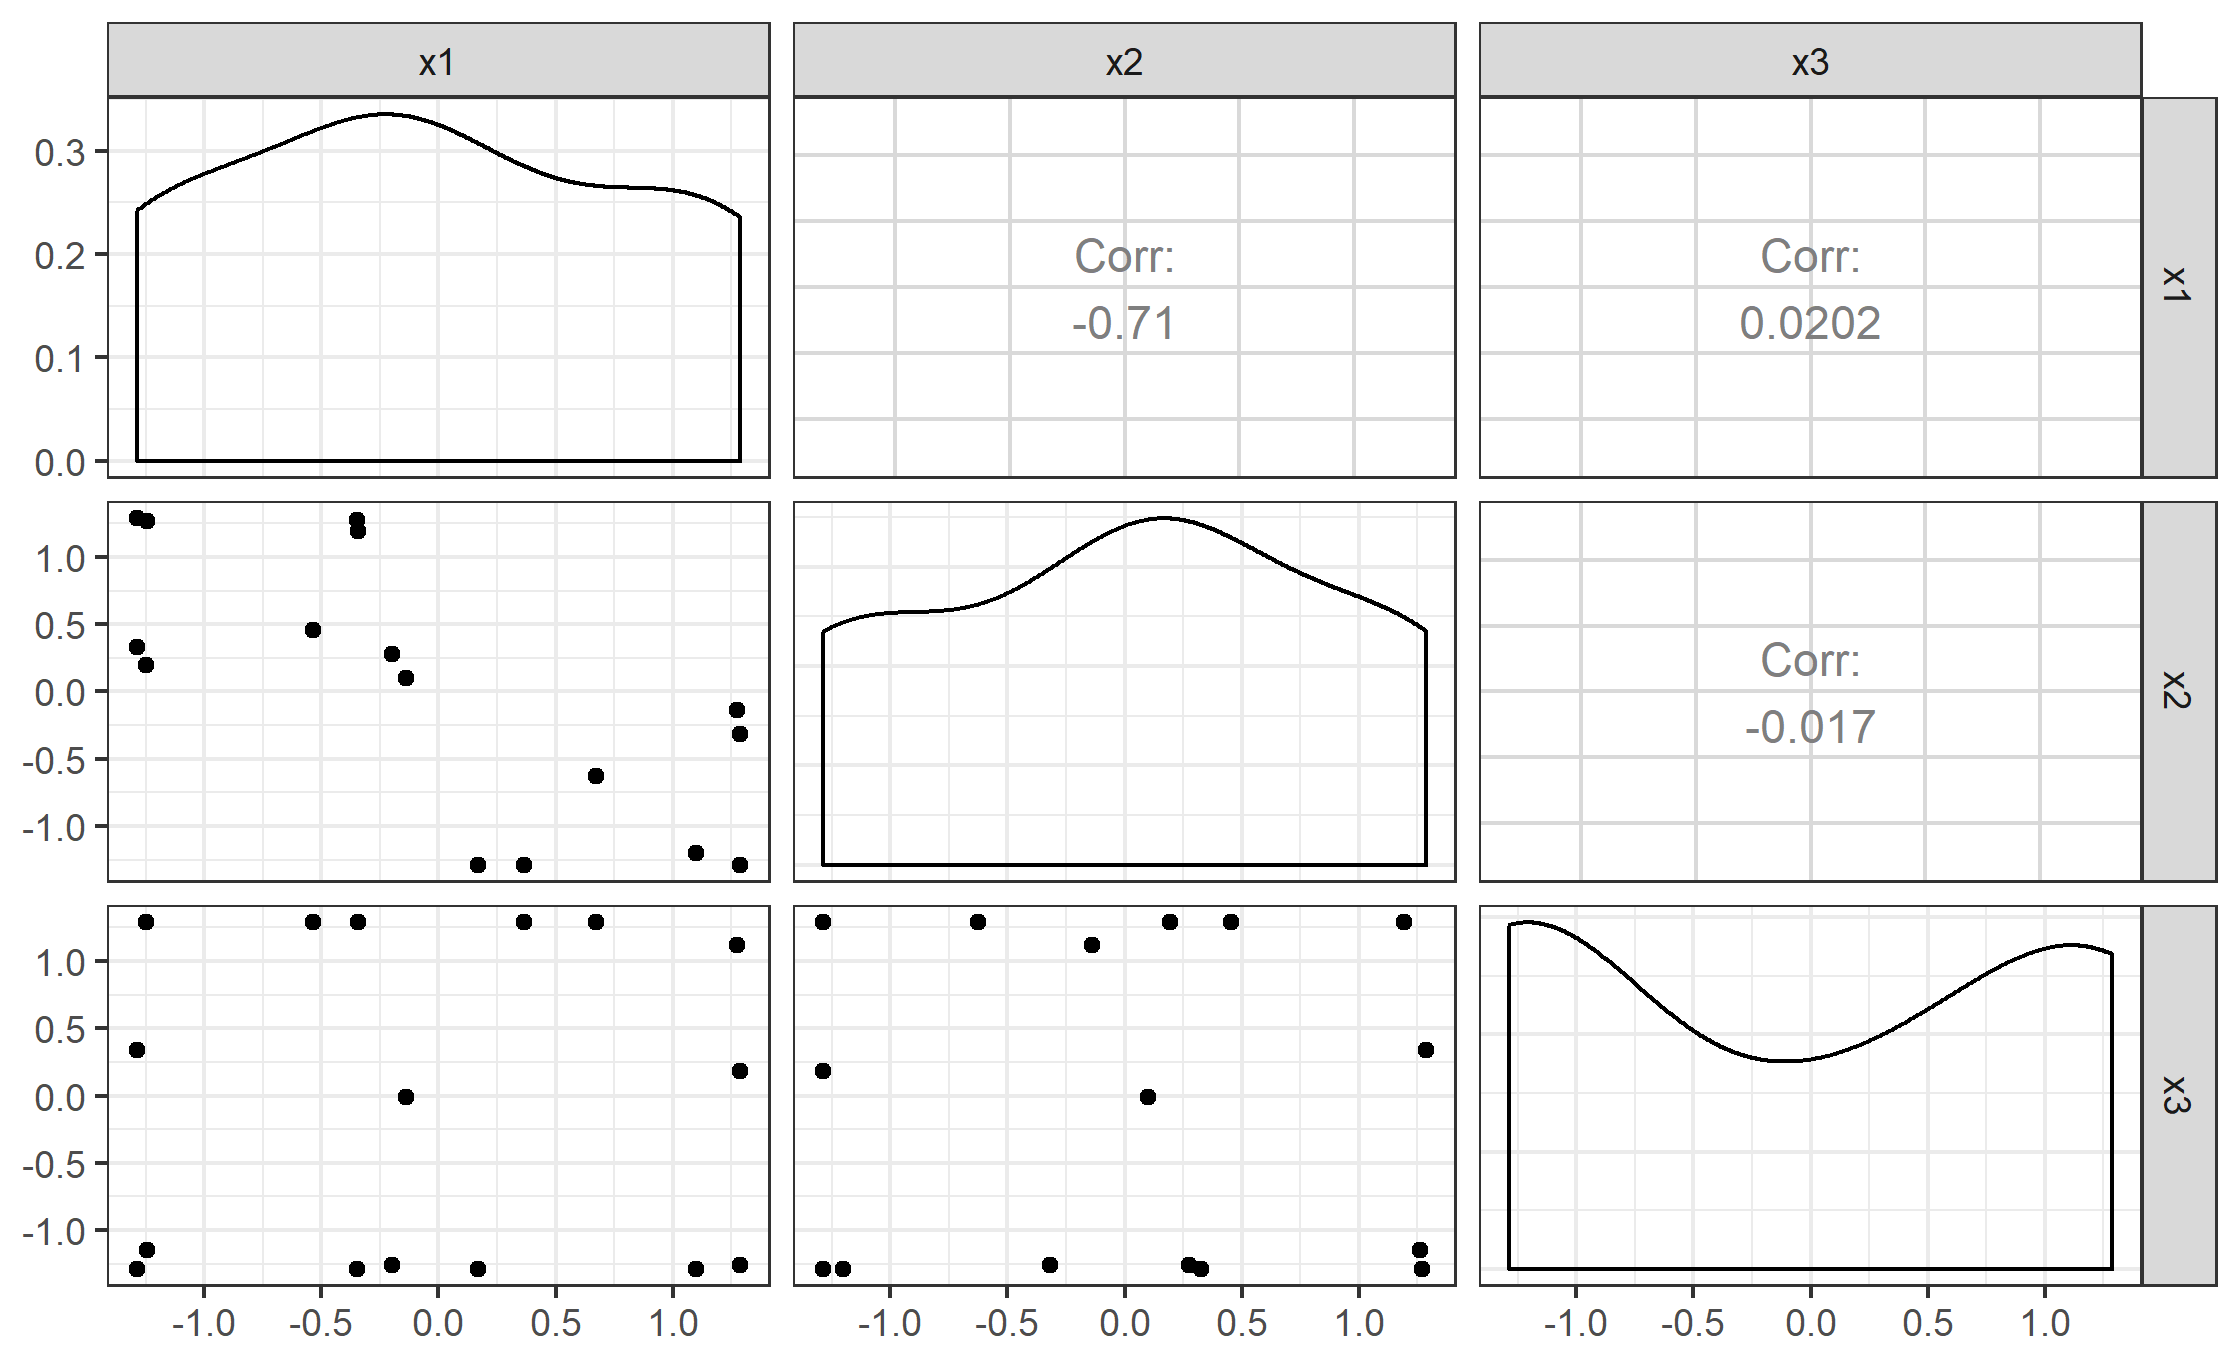
\includegraphics[width=\textwidth]{log_reg_fig_original}
    \caption{Se muestran proyecciones en una y dos dimensiones de las tres variables del modelo de regresión logística (\ref{eq:mod1_logistic_regression1}), así como su correlación.}
    \label{fig:log_reg_doe}
\end{figure}



Para corroborar la convergencia del algoritmo, la Figura \ref{fig:log_reg_conv} muestra una aproximación a la pérdida esperada del diseño en cuestión para cada una de las iteraciones de éste. Es inmediato observar que la pérdida esperada es prácticamente igual para las últimas iteraciones, lo que indica que, en efecto, el método convergió.


\begin{figure}[h]
	\centering
    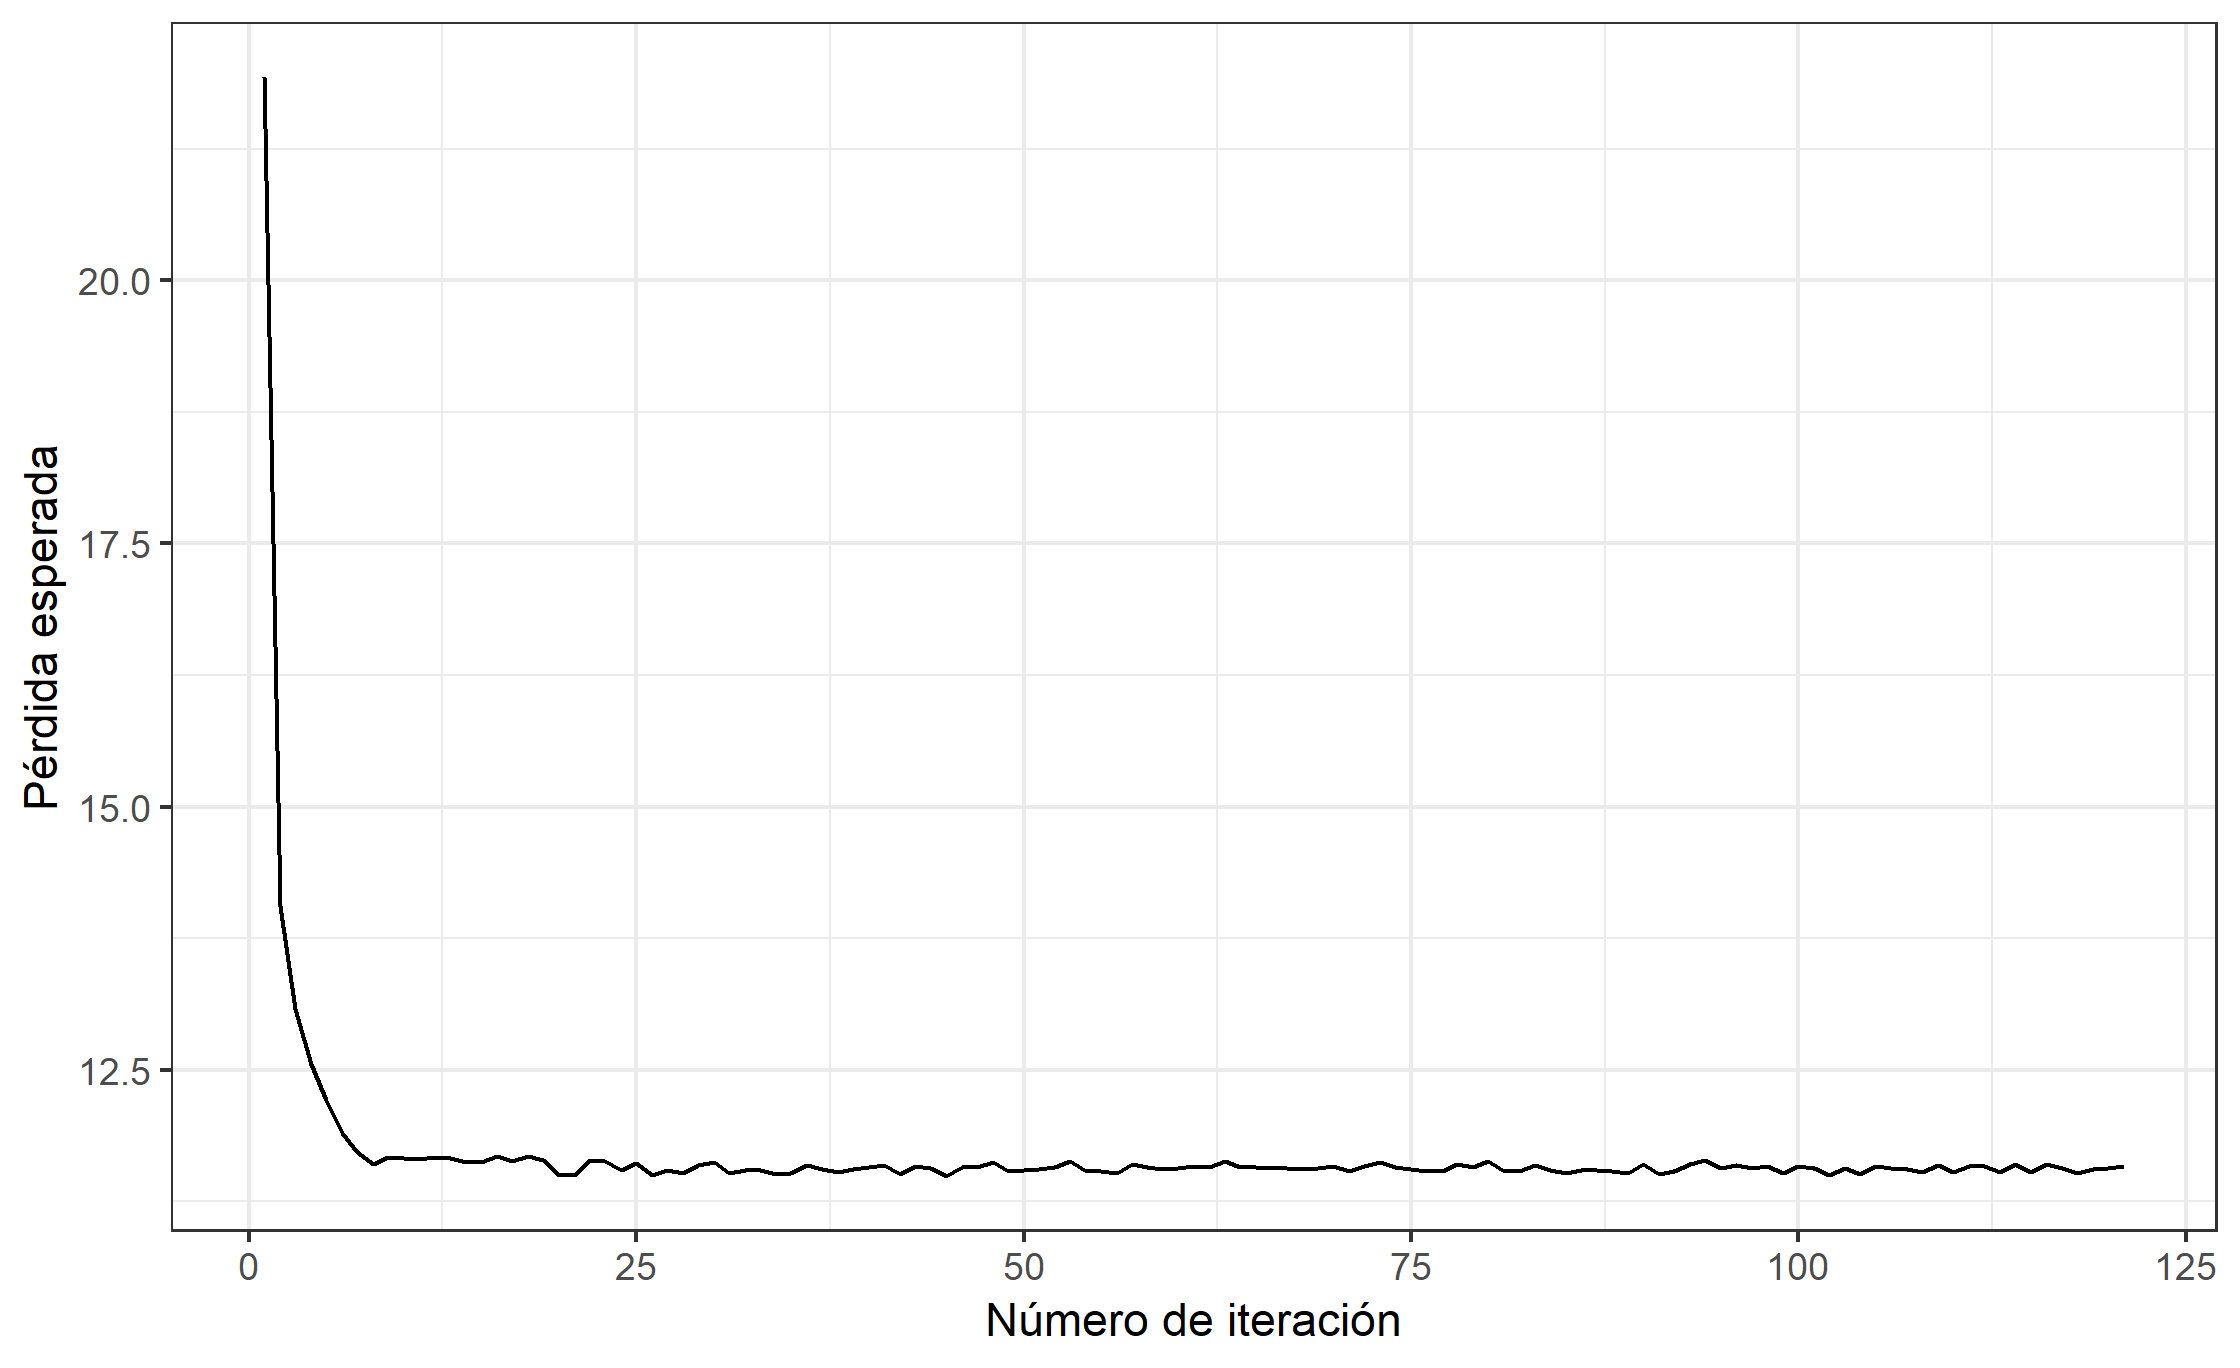
\includegraphics[width=\textwidth]{fig_conv_log_reg_original}
    \caption{Para la regresión logística (\ref{eq:mod1_logistic_regression1}), se muestran aproximaciones a la utilidad esperada de los diseños en cada iteración del algoritmo para corroborar convergencia.}
    \label{fig:log_reg_conv}
\end{figure}



\FloatBarrier


Para bosquejar la complejidad del problema es posible preguntarse qué forma toma la pérdida esperada. Dado que se encontró el diseño $D$~-óptimo Bayesiano, la pérdida esperada que este diseño minimiza está dada por
\begin{equation*}
	\Phi_{\text{D}} (\mathbf{x}) = \int_{\mathcal{Y}} \int_{B} \log \left( \frac{1}{p(\beta \, | \, y, \mathbf{x})} \right) p( \beta, y \, | \, \mathbf{x} ) \,d\beta \,dy,
\end{equation*}
donde $B = S_1 \times S_2 \times \cdots \times S_{10}$ es el espacio parametral y $S_i$ se refiere al soporte de $\beta_i$ (uno de (2, 6) o (-2,2)). Hay dos factores que entran en juego en este caso: la distribución posterior de $\beta$ y la distribución conjunta de $\beta$ e $y$. \\

La distribución posterior de $\beta$ depende tanto del diseño en cuestión $\mathbf{x}$ como de los datos $y$ que se observarán al realizar el experimento en las condiciones especificadas por $\mathbf{x}$. Por lo mismo no es inmediato obtener una expresión para $p(\beta \, | \, y, \mathbf{x})$, sino que se debe emplear el teorema de Bayes:
\begin{equation*}
	p(\beta \, | \, y, \mathbf{x}) = \frac{p(y \, | \, \beta, \mathbf{x}) \, p(\beta)}{p(y \, | \, \mathbf{x})}.
\end{equation*}
Esta expresión a su vez se divide en tres factores:
\begin{enumerate}
	\item $p(y \, | \, \beta, \mathbf{x})$ es la verosimilitud. Dado que los datos provienen independientemente de una distribución Bernoulli se tiene que
    \begin{align*}
    	p(y \, | \, \beta, \mathbf{x}) &= \prod_{i=1}^{16} \pi(\mathbf{x}_i)^{y_i} \, (1 - \pi(\mathbf{x}_i))^{1 - y_i} \\
        &= \prod_{i=1}^{16} \left( \frac{1}{1 + e^{-\eta_i}} \right)^{y_i} \, \left(1 - \frac{1}{1 + e^{-\eta_i}}  \right)^{1 - y_i}.
    \end{align*}
    No es posible simplificar esta expresión sin conocer los valores de los predictores, $\eta_i$.
    \item $p(\beta)$ es la distribución inicial conjunta de los parámetros. Por la independencia y distribuciones iniciales marginales de estos se tiene que
    \begin{align*}
    	p(\beta) &= \prod_{i=1}^{10} p(\beta_i) \\
        		 &= \left( \frac{1}{4} \right)^{10} \, \prod_{i=1}^{10} \mathds{1}_{S_i}(\beta_i),
    \end{align*}
    donde $\mathds{1}$ es la función indicadora.
    \item $p(y \, | \, \mathbf{x})$ es la función de densidad de los datos $y$, la cual se obtiene multiplicando las distribuciones de los puntos 1. y 2. e integrando sobre el espacio parametral $B$.
\end{enumerate}


La distribución conjunta de $\beta$ e $y$ también depende del diseño en cuestión y de los datos observados. Puntualmente
\begin{equation*}
	p( \beta, y \, | \, \mathbf{x} ) = p(\beta \, | \, y, \mathbf{x}) \, p(y \, | \, \mathbf{x}).
\end{equation*}
Esta expresión se divide a su vez en dos expresiones más, las cuales ya fueron discutidas previamente. Luego, para obtener la distribución conjunta es necesario \textit{(i)} obtener la distribución posterior de $\beta$ conjuntando los puntos 1. a 3., \textit{(ii)} obtener la densidad de $y$ dado $\mathbf{x}$ con el punto 3. y \textit{(iii)} multiplicar ambas distribuciones. \\


Habiendo obtenido estas componentes es aún necesario calcular el logaritmo del recíproco de la distribución posterior de $\beta$, multiplicarlo por la distribución conjunta de $\beta$ e $y$ y, posteriormente, evaluar la integral sobre todo el espacio parametral y luego sobre todo el espacio muestral. Si se quisiera encontrar el diseño óptimo entonces tendría que encontrarse analíticamente el mínimo de dicha expresión. \\

Evaluar la integral y minimizarla es claramente imposible, pero incluso tratar de obtener una expresión para el integrando es claramente una tarea compleja. Es por ello que, si se desean encontrar diseños no triviales, se \textit{debe} recurrir a herramientas computacionales como el método ACE. \\






Hay un punto que merece mayor discusión. La distribución inicial empleada por los autores para $\beta_1$ y $\beta_2$ es una distribución $\U (2, 6)$. Notoriamente el cero \textit{no} está contenido en el soporte de esta distribución. Lo que ello implica es que, al momento de obtener datos y conjuntar esta distribución inicial con la verosimilitud para así obtener la distribución final, el cero tampoco estará contenido en el soporte de la distribución final. En otras palabras, los autores están suponiendo que tanto $\beta_1$ como $\beta_2$ son diferentes de cero a priori. Y, más aún, este supuesto no cambiará independientemente de los datos observados. \\


Por otro lado, ni \cite{Woods_etal_2006} ni \cite{Woods_etal} dan alguna explicación clara sobre por qué supusieron que dichos coeficientes son distintos de cero. Por ello se volvió a encontrar el diseño $D$~-óptimo Bayesiano pero cambiando las distribuciones iniciales de estos dos parámetros, de forma que éstas fueran
\begin{align} \label{eq:mod1_params_initial_modified}
\begin{split}
	\beta_1, \beta_2 &\sim \U (-2, 6). 
\end{split}
\end{align}

No hay razón para modificar las demás distribuciones iniciales, ya que éstas sí contienen al cero en su soporte. Además, se dejó igual el límite superior del intervalo de $\beta_1$ y $\beta_2$, pero se modificó el límite inferior de forma que éste coincidiera con el de las demás distribuciones. Se utilizaron los mismos parámetros del método ACE que en el ejemplo anterior, es decir, $B=1,000$ y $Q = 10$ en el método ACE (Código \ref{code:ACE_Method}) y $\tilde{B} = 20,000$ en el algoritmo de aceptación y rechazo (Código \ref{code:ACE_AcceptReject}). La matriz de diseño óptima es
\begin{equation} \label{eq:logistic_regression_opt_design_modified}
	X_{\text{Modificada}}^{*} = \begin{bmatrix}
			    1.29 & -1.29 &  1.23 \\
			    1.29 & -1.27 & -1.27 \\
			    0.12 & -0.19 & -1.23 \\
			    0.44 & -1.29 &  0.06 \\
			    0.18 &  1.29 & -1.29 \\
			   -1.29 &  0.89 &  1.29 \\
			    1.27 &  0.55 & -1.27 \\
			   -1.15 &  1.29 & -1.11\\
			   -0.16 &  0.66 &  1.25\\
			   -0.33 &  0.13 & -0.05 \\
			    1.28 &  1.29 &  1.29 \\
			   -0.44 & -1.29 & -1.29 \\
			   -1.29 & -0.03 & -1.29 \\
			   -1.29 & -0.86 &  1.21 \\
			    0.09 & -0.46 &  1.29 \\
			    1.13 & -0.09 &  0.42
	      \end{bmatrix}
\end{equation}

Es de observar que el hecho de modificar las distribuciones iniciales derivó en un diseño óptimo diferente. Para obtener conclusiones de mayor profundidad la Figura \ref{fig:log_reg_doe_modified} es análoga a la Figura \ref{fig:log_reg_doe}, y muestra las proyecciones de las variables en una y dos dimensiones (con un suavizamiento para mostrar densidad en la primera de ellas) y las correlaciones. \\







\begin{figure}[h]
	\centering
    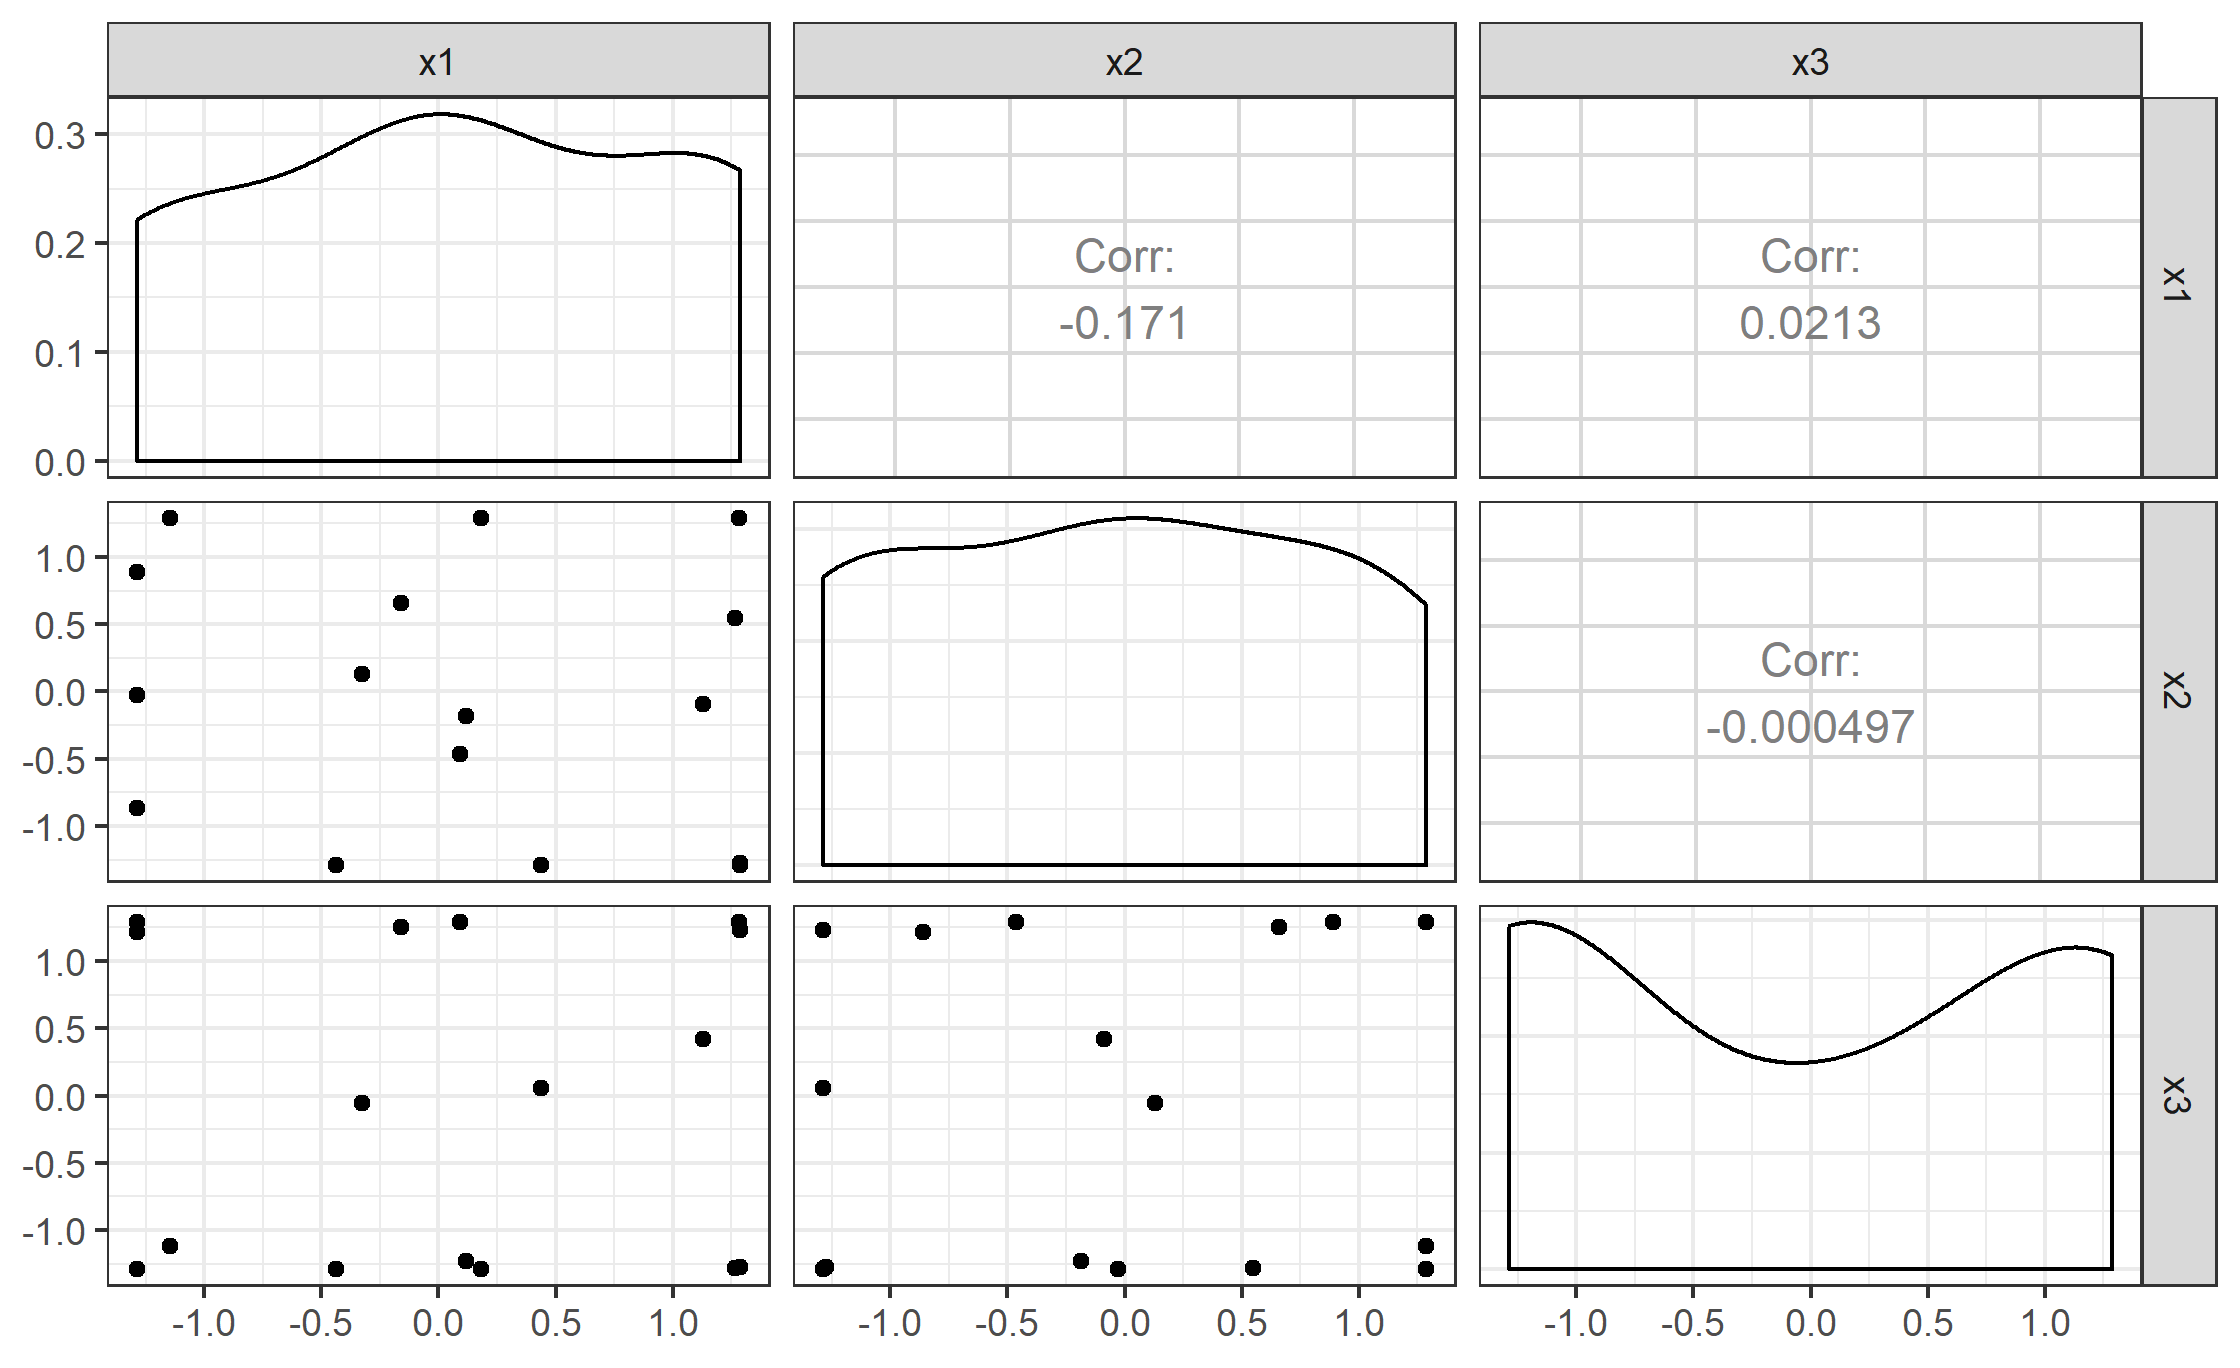
\includegraphics[width=\textwidth]{log_reg_fig_modified}
    \caption{Se muestran proyecciones en una y dos dimensiones de las tres variables del modelo de regresión logística (\ref{eq:mod1_logistic_regression1}) con distribuciones iniciales modificadas (\ref{eq:mod1_params_initial_modified}), así como su correlación.}
    \label{fig:log_reg_doe_modified}
\end{figure}








Hay algunas diferencias con respecto al diseño óptimo original que comentar. Primeramente la covariable $x_3$ sufrió pocos cambios, en tanto que su densidad suavizada se mantuvo prácticamente igual y sigue concentrada en los extremos del espacio muestral. En el caso de $x_2$, sin embargo, la densidad pasó de estar concentrada alrededor del cero a estar distribuida uniformemente en el espacio muestral. \\


Por otro lado es interesante observar que las correlaciones entre $x_3$ y el resto de las covariables se mantuvieron relativamente similares, siendo ambas cercanas a cero. Sin embargo, la correlación entre $x_1$ y $x_2$ cambió drásticamente, puesto que dichas variables pasaron de estar altamente correlacionadas (-0.71) a estar solo un poco correlacionadas (-0.17). Resumiendo, modificar las distribuciones iniciales de $\beta_1$ y $\beta_2$ tuvo un impacto directo en $x_1$ y $x_2$, mas no en $x_3$, lo cual tiene sentido. \\



De nuevo para corroborar la convergencia del algoritmo, la Figura \ref{fig:log_reg_conv_modified} muestra una aproximación a la pérdida esperada del diseño en cuestión para cada una de las iteraciones de éste. Es inmediato observar que la pérdida esperada es prácticamente igual para las últimas iteraciones, señal de 
convergencia en el método.


\begin{figure}[h]
	\centering
    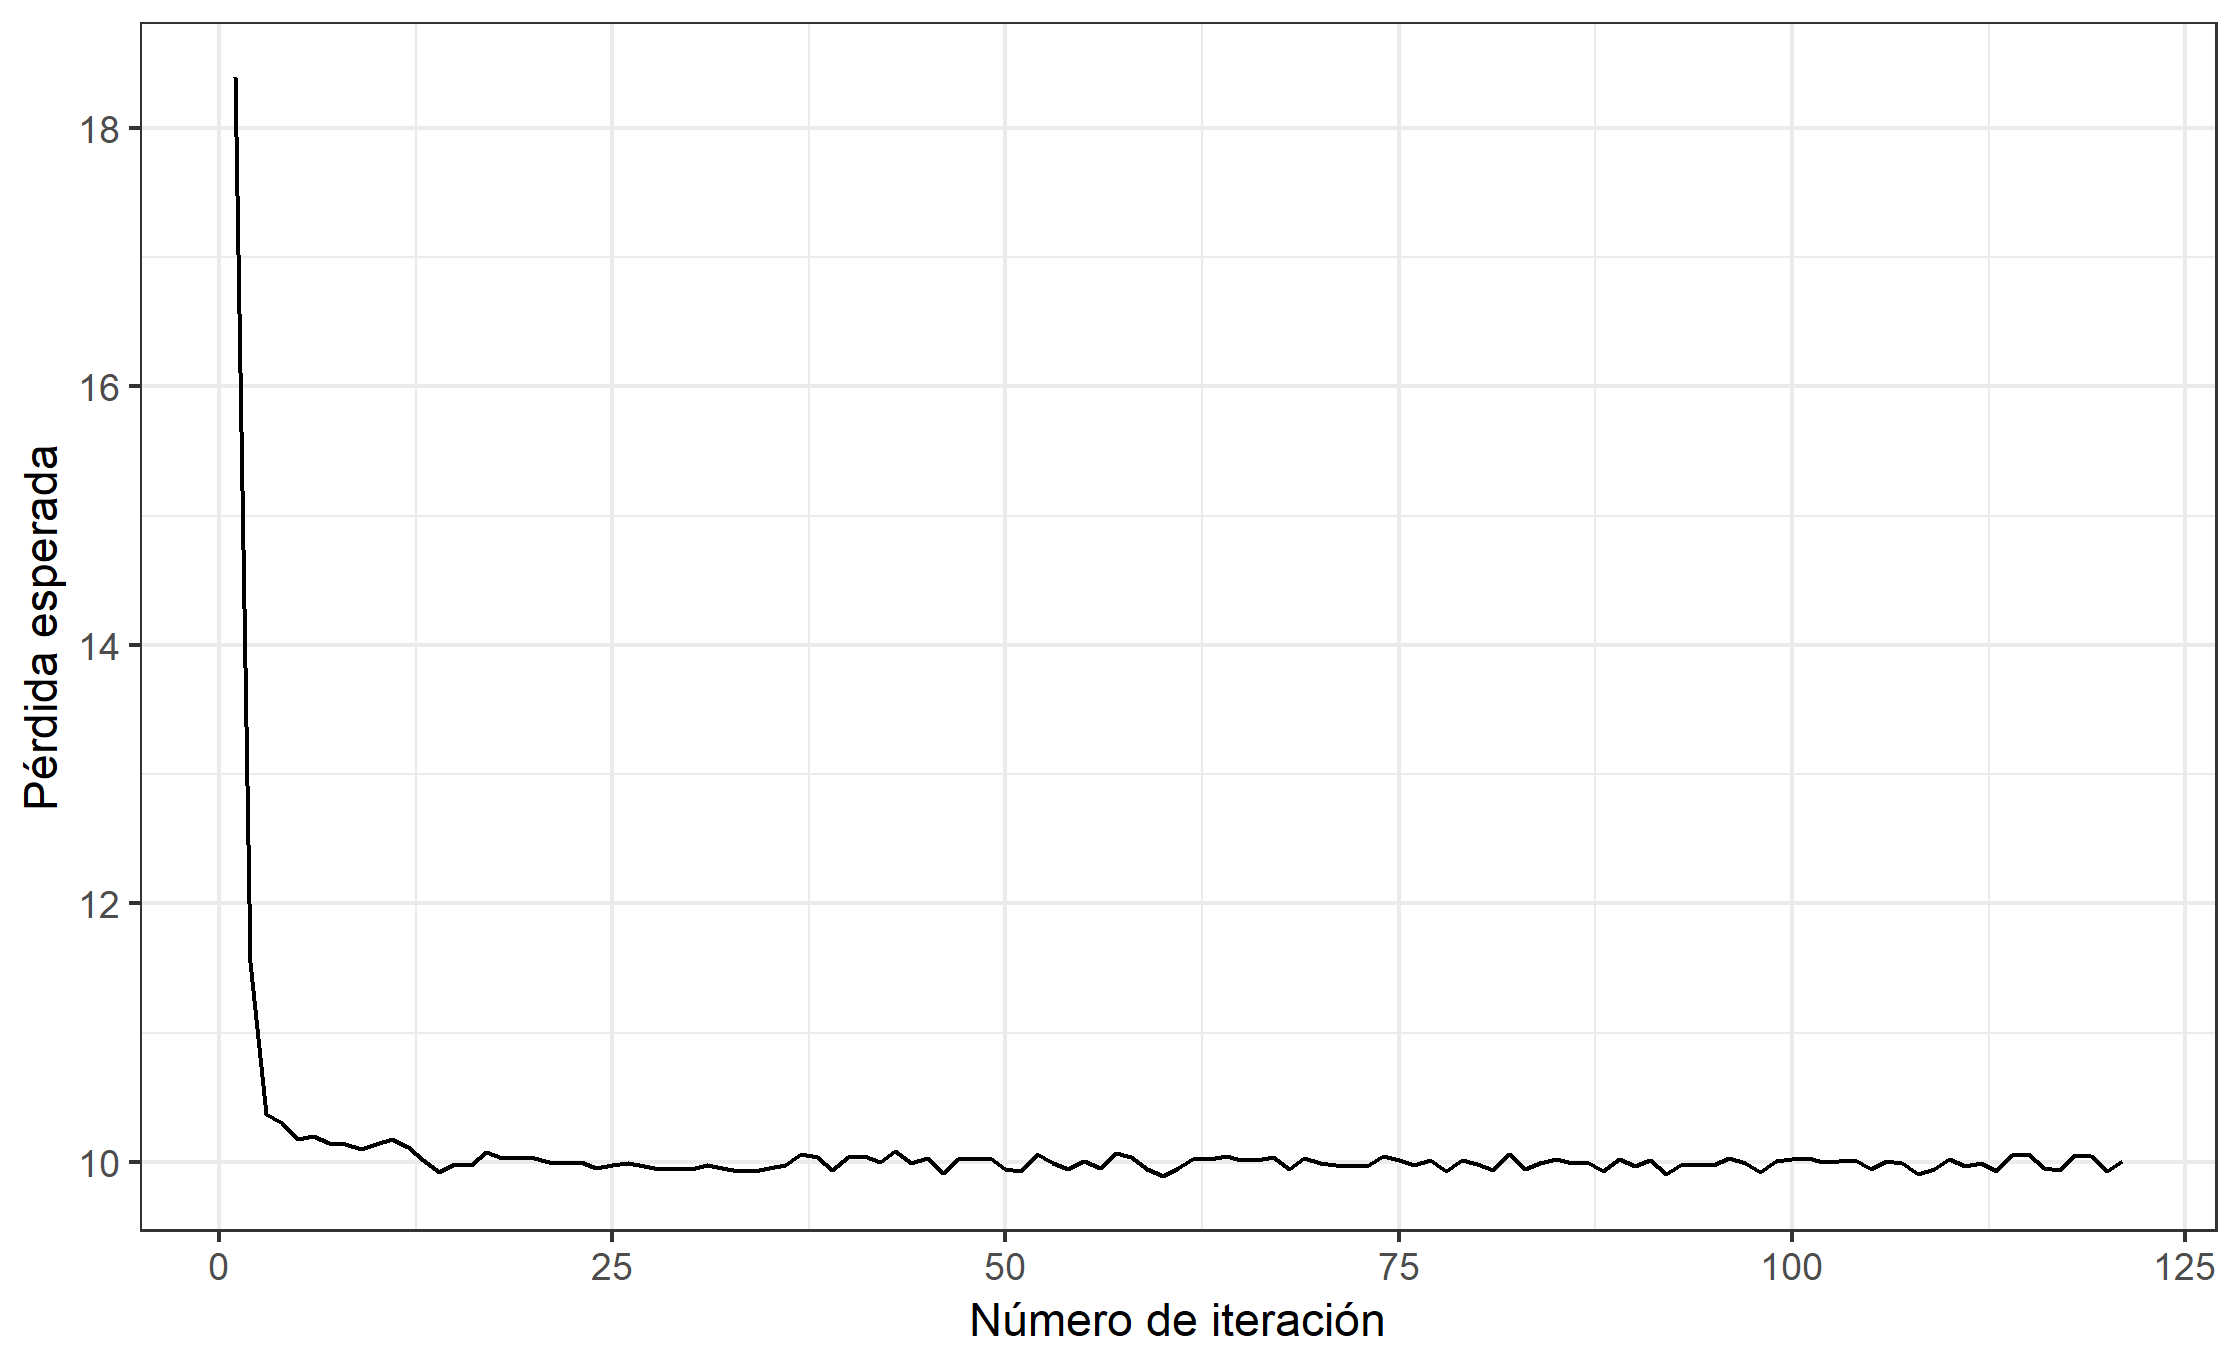
\includegraphics[width=\textwidth]{fig_conv_log_reg_modified}
    \caption{Para la regresión logística (\ref{eq:mod1_logistic_regression1}) con distribuciones iniciales modificadas (\ref{eq:mod1_params_initial_modified}), se muestran aproximaciones a la utilidad esperada de los diseños en cada iteración del algoritmo para corroborar convergencia.}
    \label{fig:log_reg_conv_modified}
\end{figure}


\FloatBarrier








\section{Diseño para modelo de regresión Poisson}



A lo largo de la historia siempre ha sido de interés modelar el número de ocurrencias de un fenómeno en cierto periodo de tiempo. La distribución Poisson es una de las alternativas más populares para este tipo de situaciones, y la familia de modelos lineales generalizados que suponen dicha distribución en la respuesta ha sido altamente estudiada. De particular interés es el modelo que utiliza la liga canónica (logarítmica), la cual se discutió con detalle en el Capítulo \ref{chapter:glms}. \\

%\newpage

\cite{atkinson_woods} encuentran resultados teóricos importantes para el diseño experimental para modelos de regresión Poisson. \cite{Woods_etal} retoman y aprovechan dichos resultados, asumiendo que se tiene un experimento con $n=6$ ensayos para cinco variables $x_1, ..., x_5$. Sea $Y_i \sim \Pois(\lambda(x_i))$. Entonces se pretende modelar
\begin{equation} \label{eq:mod2_poisson_regression1}
	\log \lambda(x_i) = \beta_0 + \sum_{j=1}^{5} \beta_j x_{ij}, \quad i=1,...,6,
\end{equation}
aprovechando que $\lambda(x_i) = \mu(x_i)$ en el modelo Poisson.\\


Más aún, los autores asumen que $\beta_0 = 0$ es conocido. 	Las distribuciones iniciales para los demás parámetros son independientes y están dadas por
\begin{align} \label{eq:mod2_params_initial}
\begin{split}
	\beta_1, \beta_3, \beta_5 &\sim \mathcal{U}(1, 1+\alpha),\\
    \beta_2, \beta_4 &\sim \mathcal{U}(-1-\alpha, -1),
\end{split}
\end{align}
donde $\alpha > 0$ es un parámetro fijo. Las covariables toman valores en $[-1, 1]^5$, utilizando la notación del ejemplo anterior. Los demás argumentos del método ACE utilizados por los autores son $B=1,000$ y $Q = 20$ en el método ACE (Código \ref{code:ACE_Method}) y $\tilde{B} = 20,000$ en el algoritmo de aceptación y rechazo (Código \ref{code:ACE_AcceptReject}). \\

Woods et al. encuentran el diseño SIL-óptimo para los valores ${\alpha = 0.5}$ y ${\alpha = 0.75}$. Para comparar con sus resultados se encontró el diseño $D$~-óptimo.
La Tabla \ref{table:alfa5} muestra la comparación del diseño SIL-óptimo con el $D$~-óptimo para $\alpha = 0.5$, y la Tabla \ref{table:alfa75} muestra lo respectivo para $\alpha = 0.75$.


\begin{table}[h]
\small
\centering
\begin{tabular}{l|lllll|lllll}
\multirow{2}{*}{Núm} & \multicolumn{5}{l|}{ \hspace{1.2cm} Diseño $D$~-óptimo} & \multicolumn{5}{l}{  \hspace{1cm}  Diseño SIL-óptimo}  \\
                     & $x_1$  & $x_2$ & $x_3$ & $x_4$ & $x_5$ & $x_1$ & $x_2$ & $x_3$ & $x_4$ & $x_5$  \\ \hline
1                    & -0.42  & -1    & 1     & -1    & 1     & -0.5  & -1    & 1     & -1    & 1      \\
2                    & 1      & 0.5  & 1     & -1    & 1     & 1     & 0.56  & 1     & -1    & 1      \\
3                    & 1      & -1    & -0.36  & -1    & 1     & 1     & -1    & -0.31 & -1    & 1      \\
4                    & 1      & -1    & 1     & 0.51  & 1     & 1     & -1    & 1     & 0.33  & 1      \\
5                    & 1      & -1    & 1     & -1    & -0.39 & 1     & -1    & 1     & -1    & -0.38 \\
6                    & 1      & -1    & 1     & -1    & 1     & 1     & -1    & 1     & -1    & 1     
\end{tabular}
\caption{Se muestran los diseños óptimos según los dos distintos criterios para $\alpha = 0.5$.}
\label{table:alfa5}
\end{table}



\begin{table}[h]
\small
\centering
\begin{tabular}{l|lllll|lllll}
\multirow{2}{*}{Núm} & \multicolumn{5}{l|}{ \hspace{1.2cm} Diseño $D$~-óptimo} & \multicolumn{5}{l}{  \hspace{1cm}  Diseño SIL-óptimo}  \\
                     & $x_1$  & $x_2$ & $x_3$ & $x_4$ & $x_5$ & $x_1$ & $x_2$ & $x_3$ & $x_4$ & $x_5$  \\ \hline
1                    & -0.32  & -1    & 1     & -1    & 1     & -0.22  & -1    & 1     & -1    & 1      \\
2                    & 1      & 0.34  & 1     & -1    & 1     & 1     & 0.22  & 1     & -1    & 1      \\
3                    & 1      & -1    & -0.34  & -1    & 1     & 1     & -1    & -0.32 & -1    & 1      \\
4                    & 1      & -1    & 1     & 0.38  & 1     & 1     & -1    & 1     & 0.11  & 1      \\
5                    & 1      & -1    & 1     & -1    & -0.47 & 1     & -1    & 1     & -1    & -0.31 \\
6                    & 1      & -1    & 1     & -1    & 1     & 1     & -1    & 1     & -1    & 1     
\end{tabular}
\caption{Se muestran los diseños óptimos según los dos distintos criterios para $\alpha = 0.75$.}
\label{table:alfa75}
\end{table}


En ambos casos las variables toman el mismo valor, ya sea $\pm 1$, en todos los ensayos menos uno: el que aparece en la diagonal.\footnote{Aunque en estricto sentido no se puede hablar de una diagonal, se entiende que se refiere al valor $x_{ii}$ de la covariable.} Es ahí donde se aprecian las diferencias entre ambos diseños óptimos. Si bien es cierto que los signos son todos iguales, también se vislumbran pequeñas diferencias entre los valores de las variables del diseño óptimo. En particular, $x_4$ es la covariable que muestra mayor variación para ambos valores de $\alpha$. Esto se debe a que distintos criterios de optimalidad llevan a distintos diseños óptimos. Sin embargo cabe recordar que la $D$~-optimalidad Bayesiana es similar a la SIL~-optimalidad, lo que explica que ambos diseños sean relativamente similares. \\



Las Figuras \ref{fig:pois_reg5} y \ref{fig:pois_reg75} muestran las proyecciones en dos dimensiones de las variables junto con su proyección en una dimensión (en forma de densidad), para $\alpha=0.5$ y $\alpha=0.75$. Además se muestran las correlaciones que tendrán las covariables empleando el diseño óptimo. Es interesante que éstas son todas iguales a $\pm 0.2$ para ambos valores de $\alpha$. Ello indica que el diseño óptimo de nuevo no considera utilizar covariables no correlacionadas y, más aún, que la correlación entre las variables siempre será de $\pm 0.2$. \\







\begin{figure}[h]
	\centering
    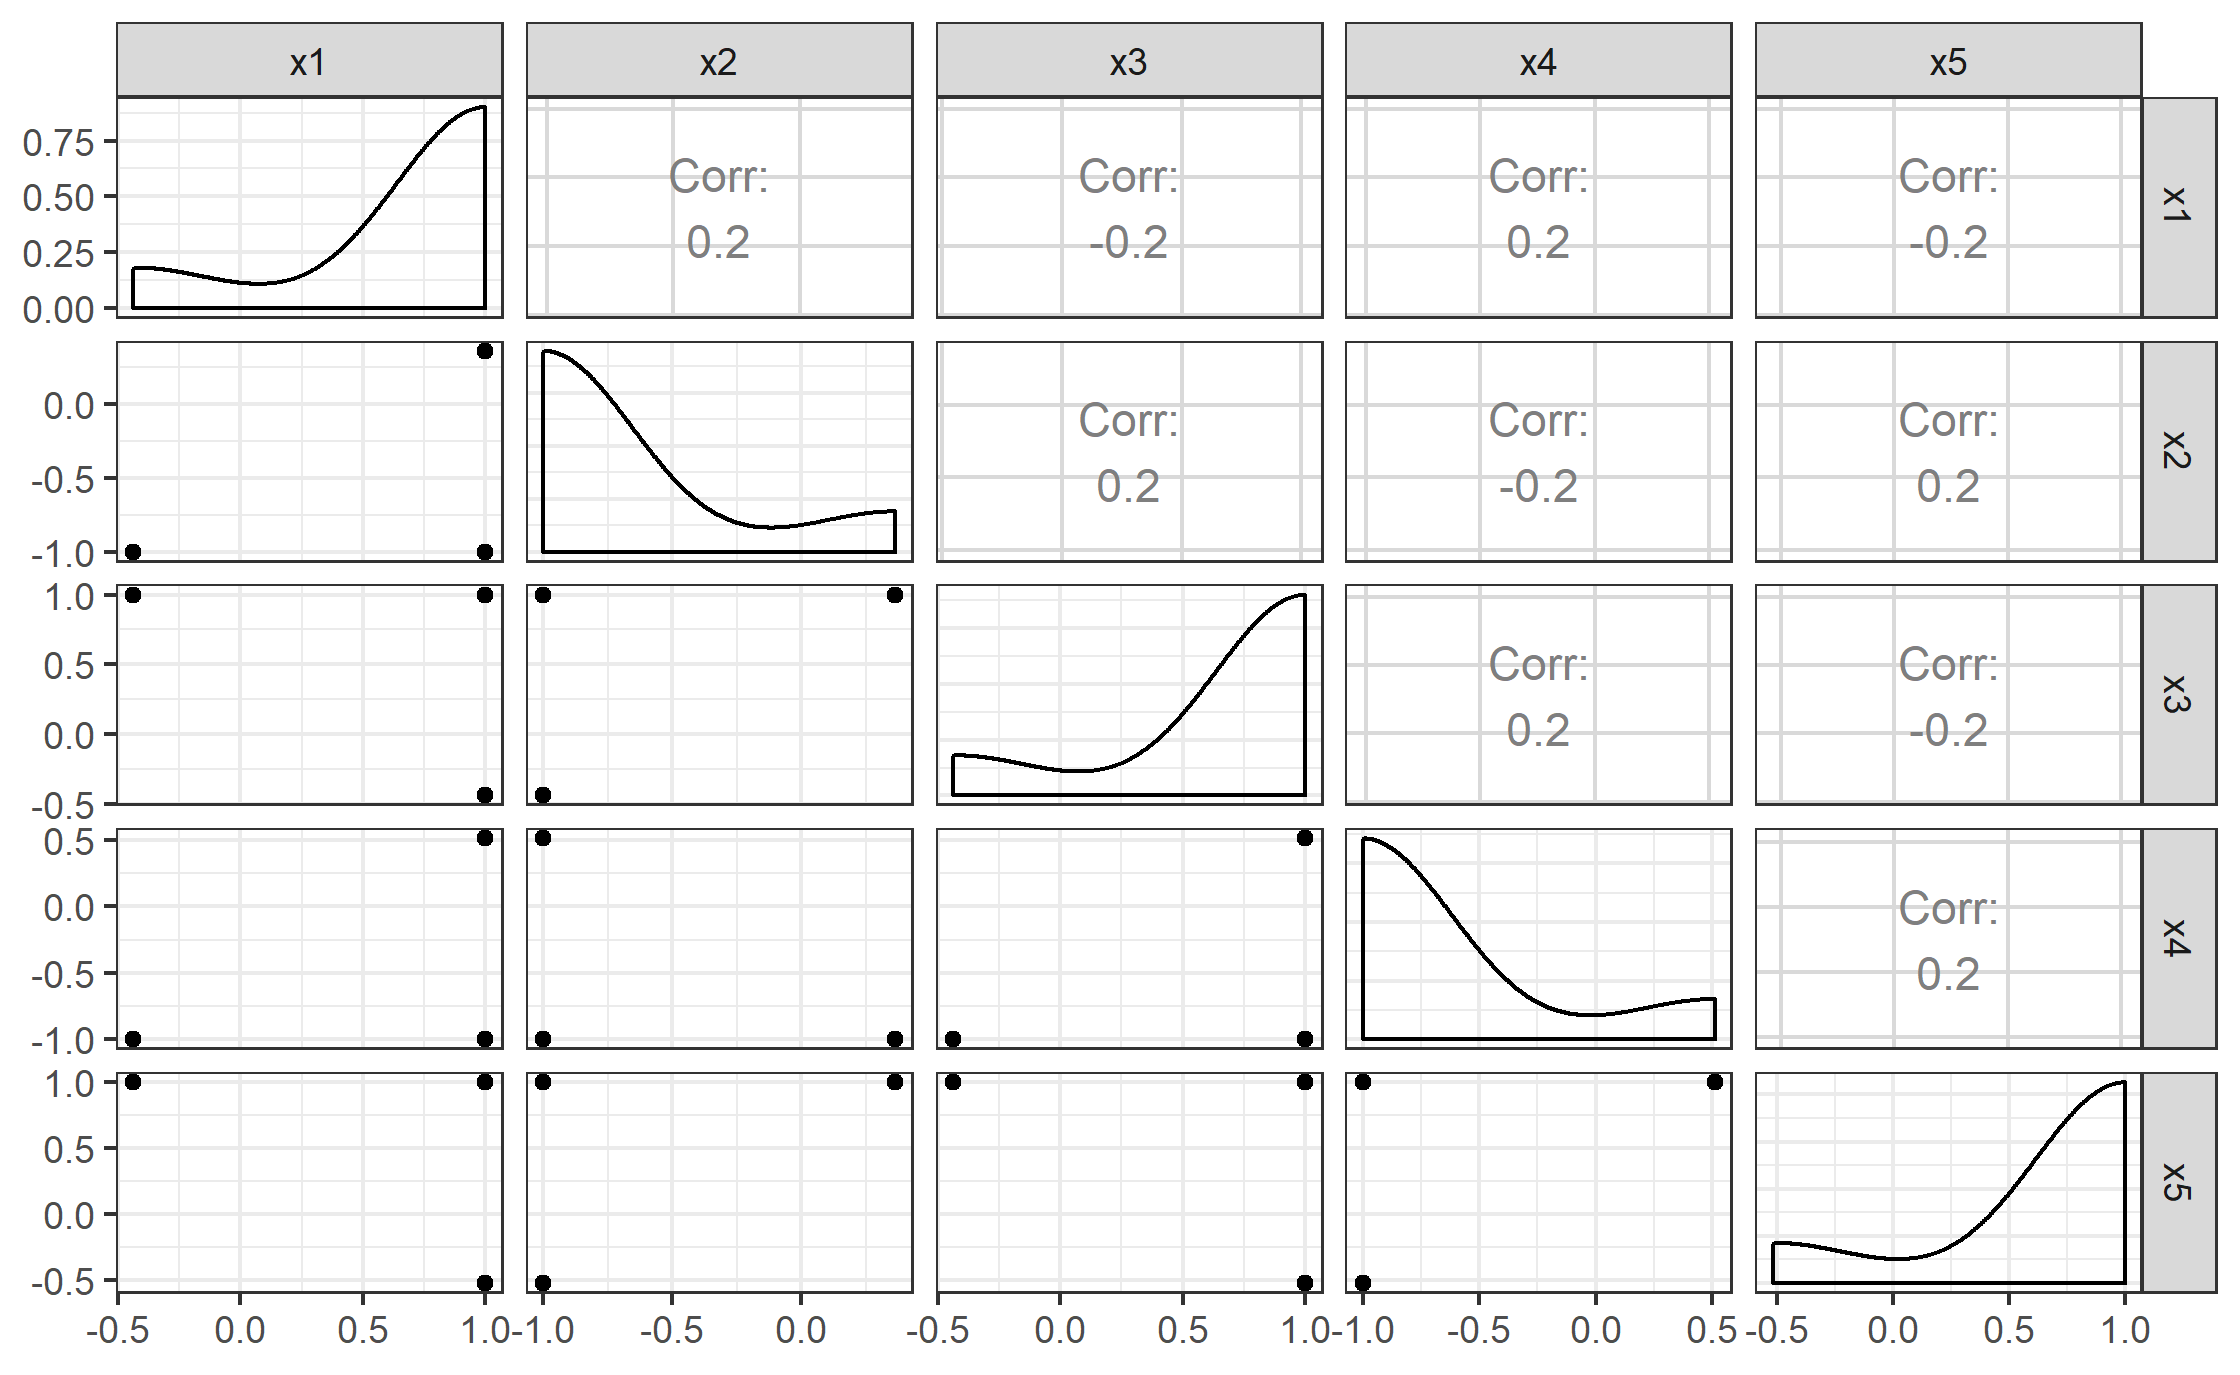
\includegraphics[width=\textwidth]{alpha_50_original.png}
    \caption{Se muestran proyecciones en una y dos dimensiones de las tres variables del modelo de regresión Poisson (\ref{eq:mod2_poisson_regression1}), así como su correlación, para $\alpha=0.5$.}
    \label{fig:pois_reg5}
\end{figure}



\begin{figure}[h]
	\centering
    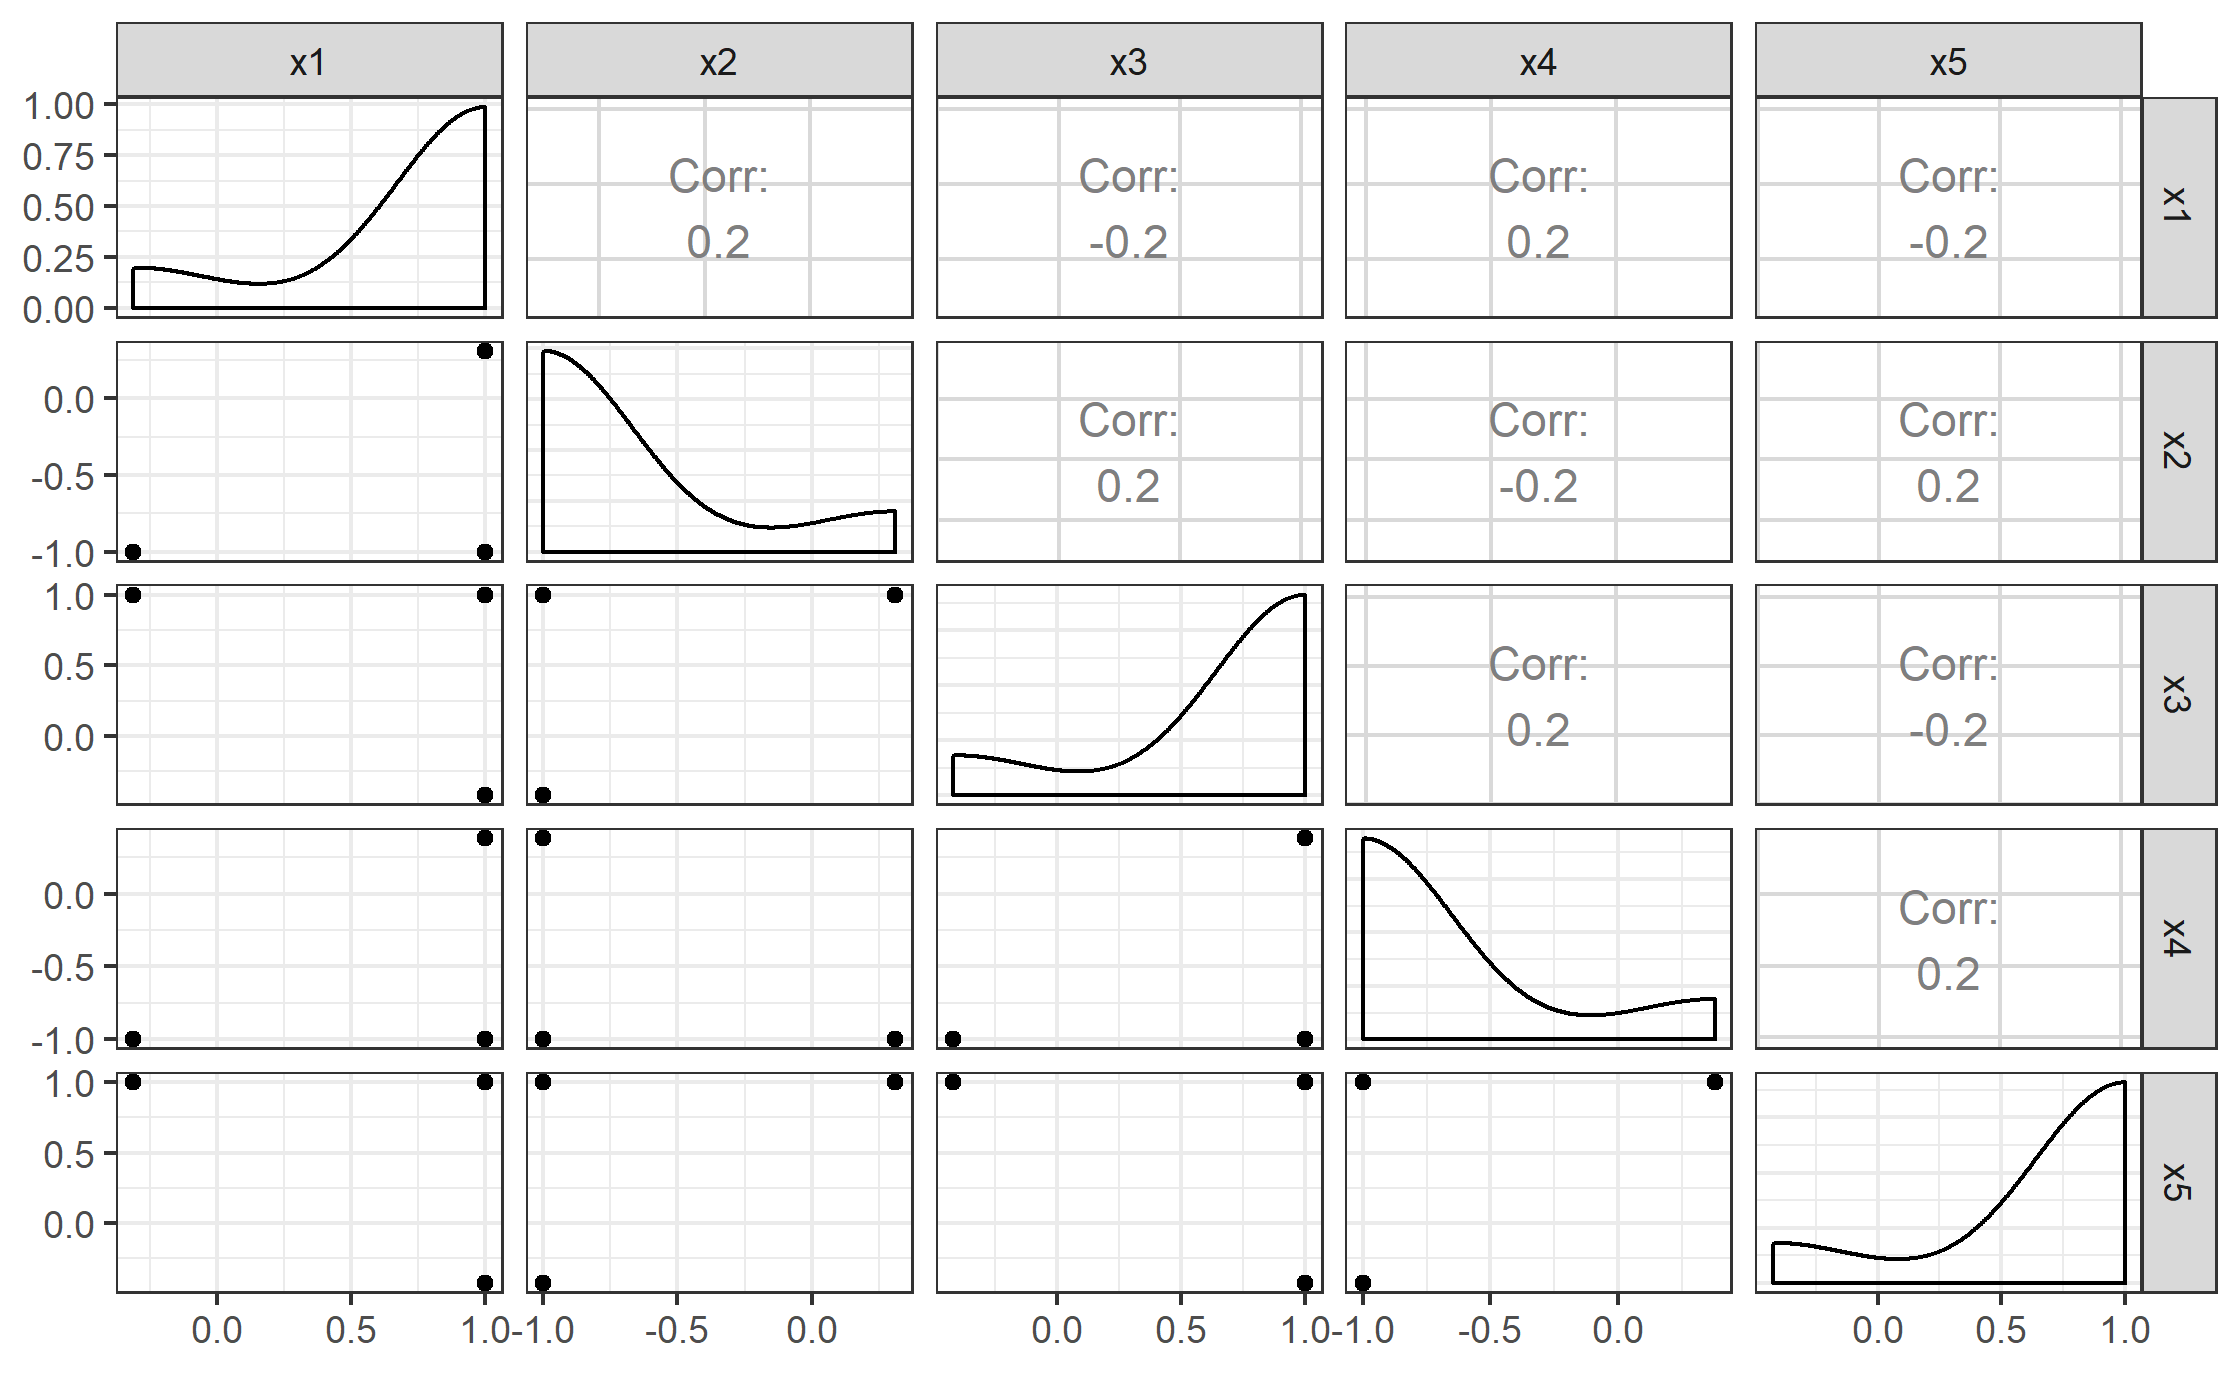
\includegraphics[width=\textwidth]{alpha_75_original.png}
    \caption{Se muestran proyecciones en una y dos dimensiones de las tres variables del modelo de regresión Poisson (\ref{eq:mod2_poisson_regression1}), así como su correlación, para $\alpha=0.75$.}
    \label{fig:pois_reg75}
\end{figure}




\begin{figure}[h]
	\centering
    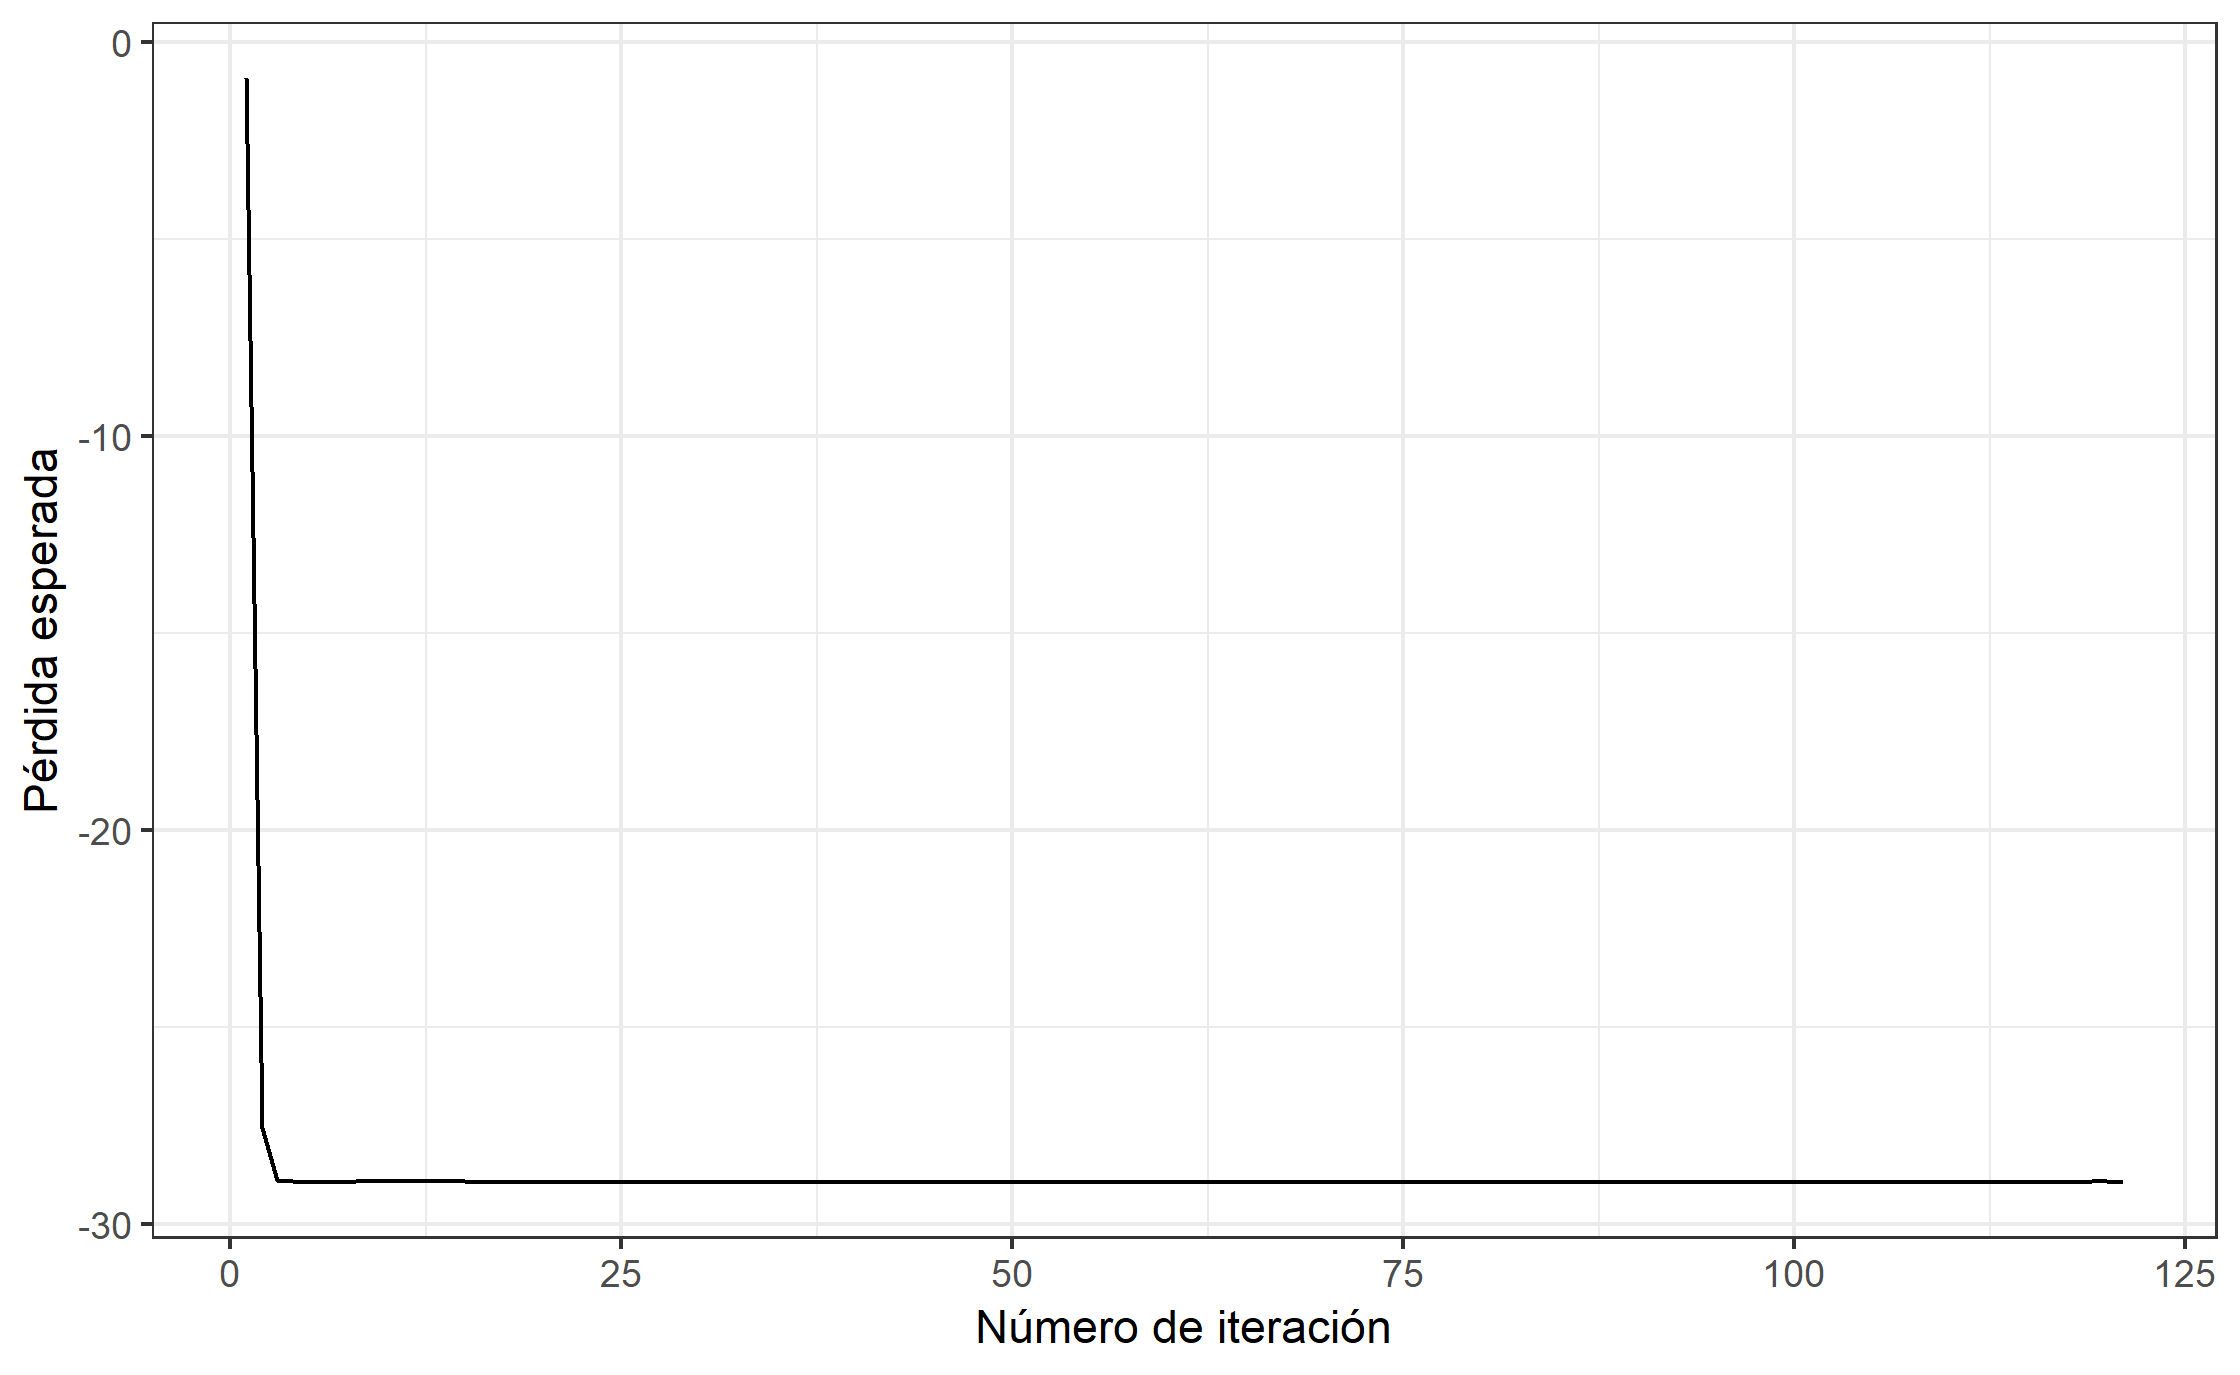
\includegraphics[width=\textwidth]{fig_conv_pois_reg_alfa5.png}
    \caption{Para la regresión Poisson con $\alpha = 0.5$, se muestran aproximaciones a la utilidad esperada de los diseños en cada iteración del algoritmo para corroborar convergencia.}
    \label{fig:pois_reg_conv_alfa5}
\end{figure}


De nuevo para corroborar la convergencia del método, las Figuras \ref{fig:pois_reg_conv_alfa5} y \ref{fig:pois_reg_conv_alfa75} muestran las aproximaciones a las utilidades esperadas del diseño en cuestión para cada iteración del algoritmo, y para $\alpha = 0.5$ y $\alpha = 0.75$, respectivamente. En ambos casos se aprecia que dichos promedios se estabilizan, por lo que se puede concluir que el método en efecto convergió.


\begin{figure}[h]
	\centering
    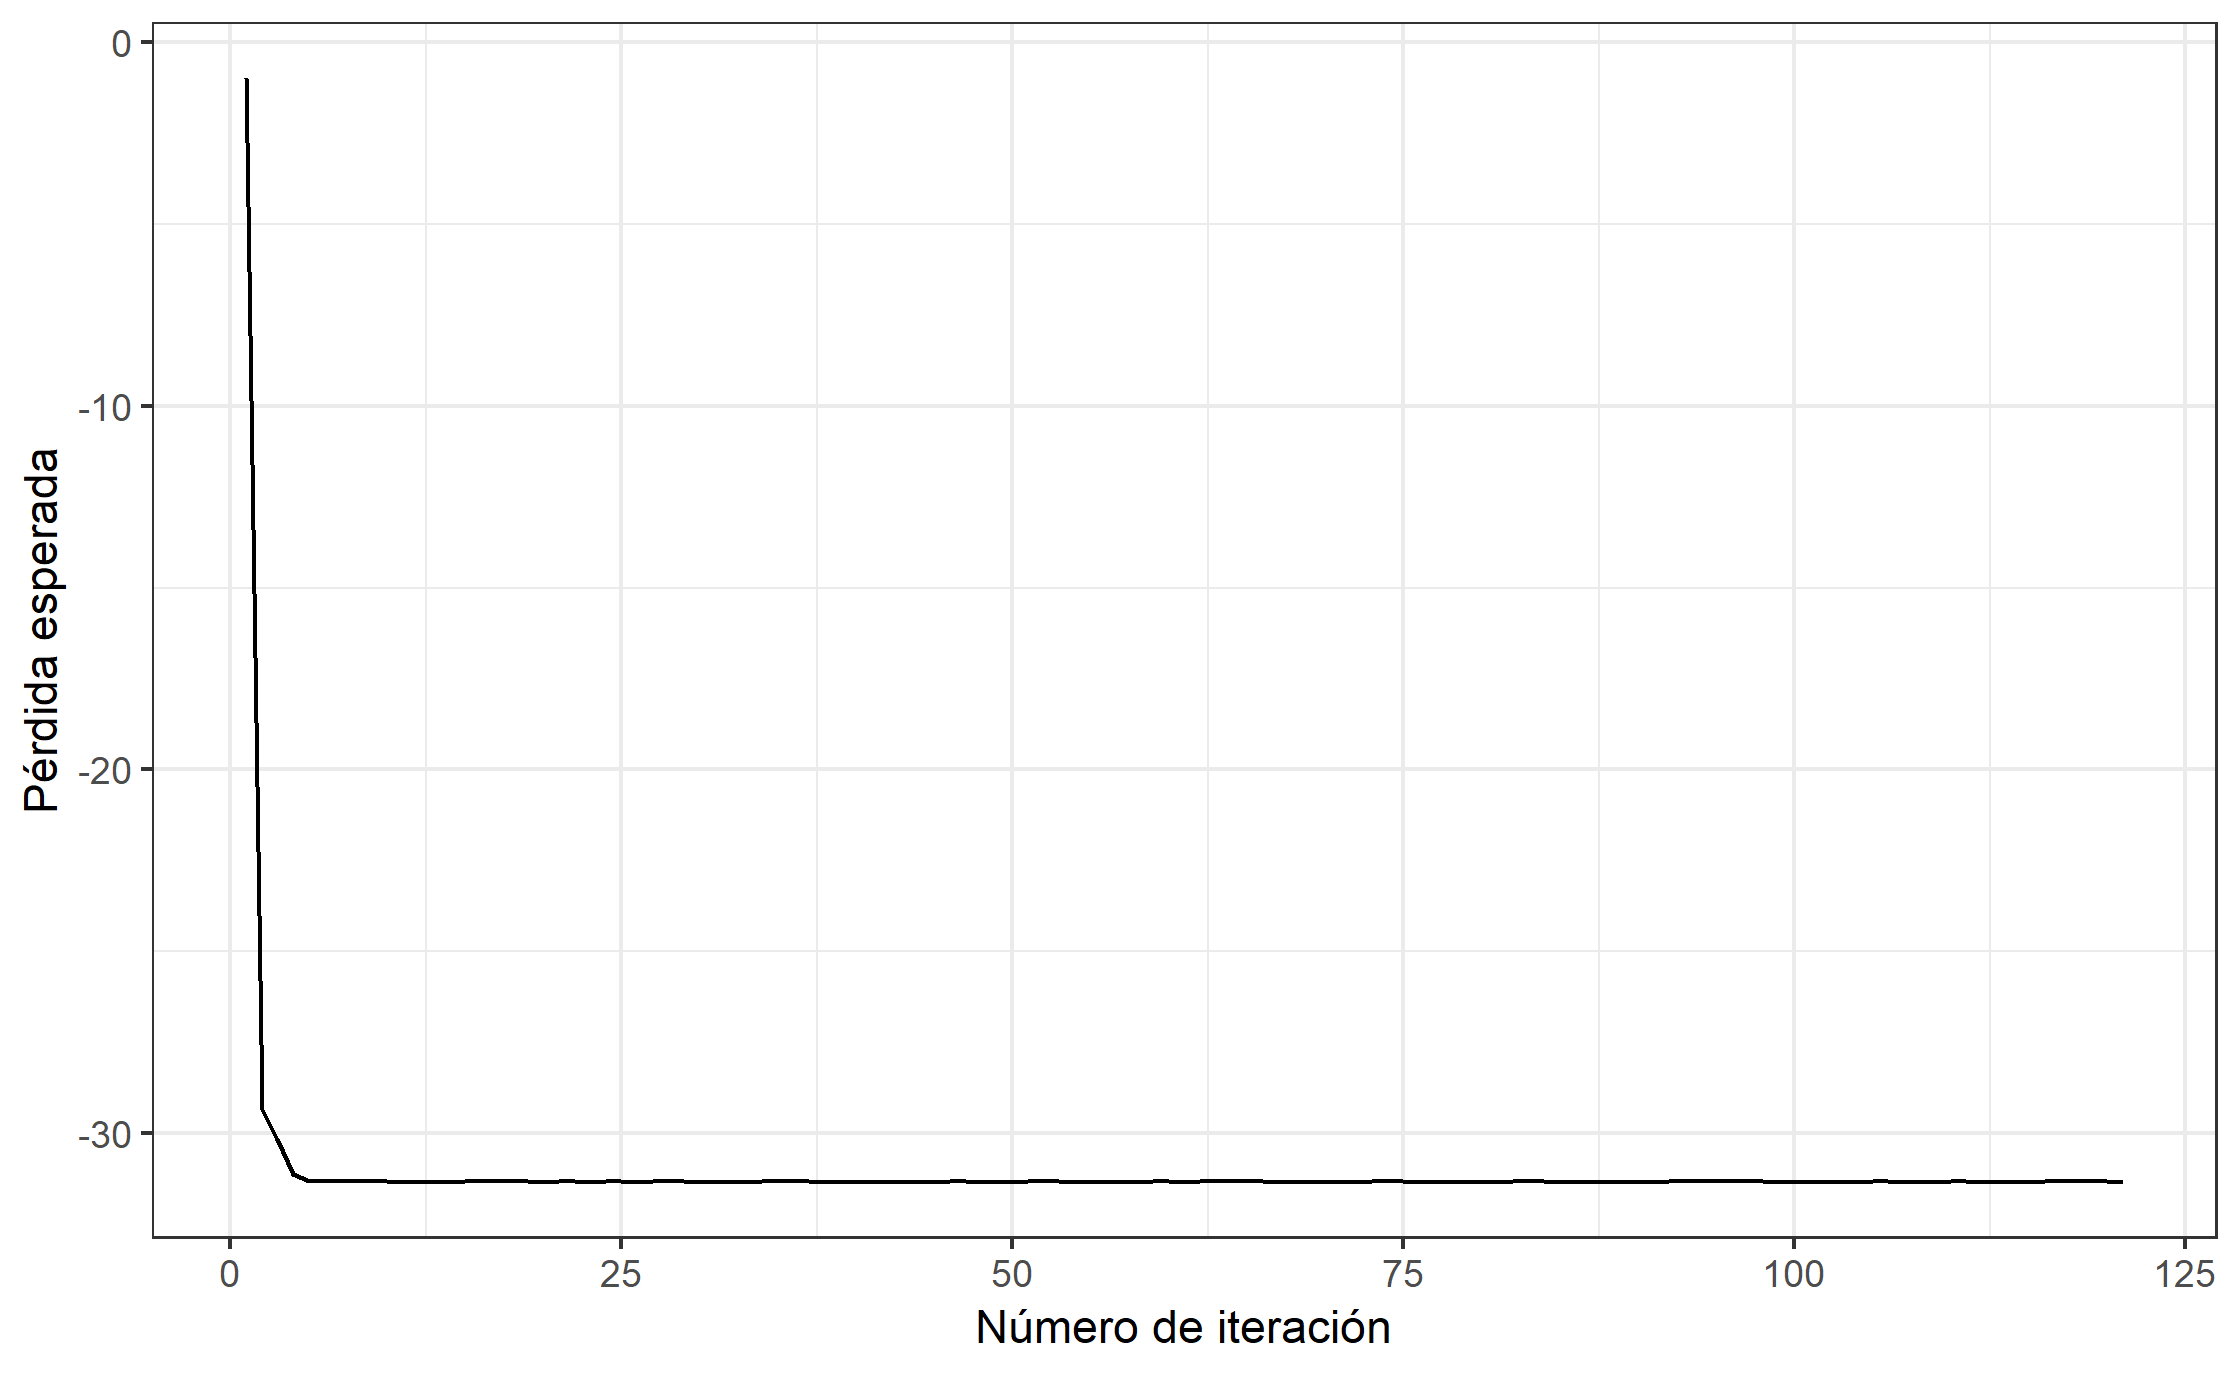
\includegraphics[width=\textwidth]{fig_conv_pois_reg_alfa75.png}
    \caption{Para la regresión Poisson con $\alpha = 0.75$, se muestran aproximaciones a la utilidad esperada de los diseños en cada iteración del algoritmo para corroborar convergencia.}
    \label{fig:pois_reg_conv_alfa75}
\end{figure}


\FloatBarrier



Otra manera de estudiar las diferencias entre los diseños $D$~-óptimos y los diseños SIL~-óptimos es comparando las distribuciones posteriores a las que dan lugar. Para ello es necesario conocer los verdaderos valores de los parámetros $\beta$, lo cual no ocurre en este caso. Sin embargo, para efectos prácticos, puede escogerse algún valor cualquiera dentro del soporte de cada parámetro y suponerlo como cierto. Aunque podría optarse por escoger la media de cada distribución, o bien la mediana o algún cuantil, para este trabajo se obtuvo una observación de cada una de las distribuciones iniciales marginales de estos parámetros; estas observaciones se fijaron y se supusieron como los valores reales de cada parámetro. Puntualmente se supuso que
\begin{align} \label{eq:beta_sim}
\begin{split}
	&\beta_1 = 1.47, \quad \beta_2 = -1.14, \quad \beta_3 = 1.24, \\
    &\beta_4 = -1.50, \quad \beta_5 = 1.41.
\end{split}
\end{align}

Es posible obtener datos simulados $y$ conjuntando los valores (\ref{eq:beta_sim}) de $\beta$ con algún diseño óptimo y utilizando la expresión del modelo (\ref{eq:mod2_poisson_regression1}). Para este ejercicio se fijó $\alpha = 0.5$ y se obtuvieron así dos series de $n=6$ datos simulados: $y_D$, correspondiente a los datos obtenidos con el diseño $D$~-óptimo, e $y_{\text{SIL}}$, correspondiente a los datos obtenidos con el diseño SIL~-óptimo. \\


Posteriormente se obtuvo, utilizando el programa \texttt{JAGS} \citep{jags}, una muestra de tamaño 10,000 de la distribución posterior de $\beta$ para cada serie de datos. La Figura \ref{fig:posterior_beta} compara las densidades marginales posteriores de cada diseño óptimo, obtenidas suavizando los datos de las muestras de cada distribución posterior. \\


Si bien las distribuciones son similares para todos los parámetros, solo en el caso de $\beta_5$ éstas son prácticamente iguales. Las distribuciones marginales posteriores de $\beta_1, \beta_2, \beta_3$, y $\beta_4$ muestran diferencias entre los diseños óptimos. \\


En el caso de $\beta_2$ y $\beta_3$ las distribuciones tienen la misma forma pero las correspondientes al diseño SIL~-óptimo están recorridas ligeramente hacia la derecha, con mayor cercanía al verdadero valor del parámetro. Las distribuciones de $\beta_1$ y $\beta_4$ son interesantes porque corresponden a valores del parámetro cercanos al extremo de su respectivo intervalo. Es notorio que las distribuciones correspondientes al diseño SIL~-óptimo tienen colas más pesadas y mayor varianza, mientras que las respectivas al diseño $D$~-óptimo están más concentradas en el extremo del intervalo.  \\



\begin{figure}[h]
	\centering
    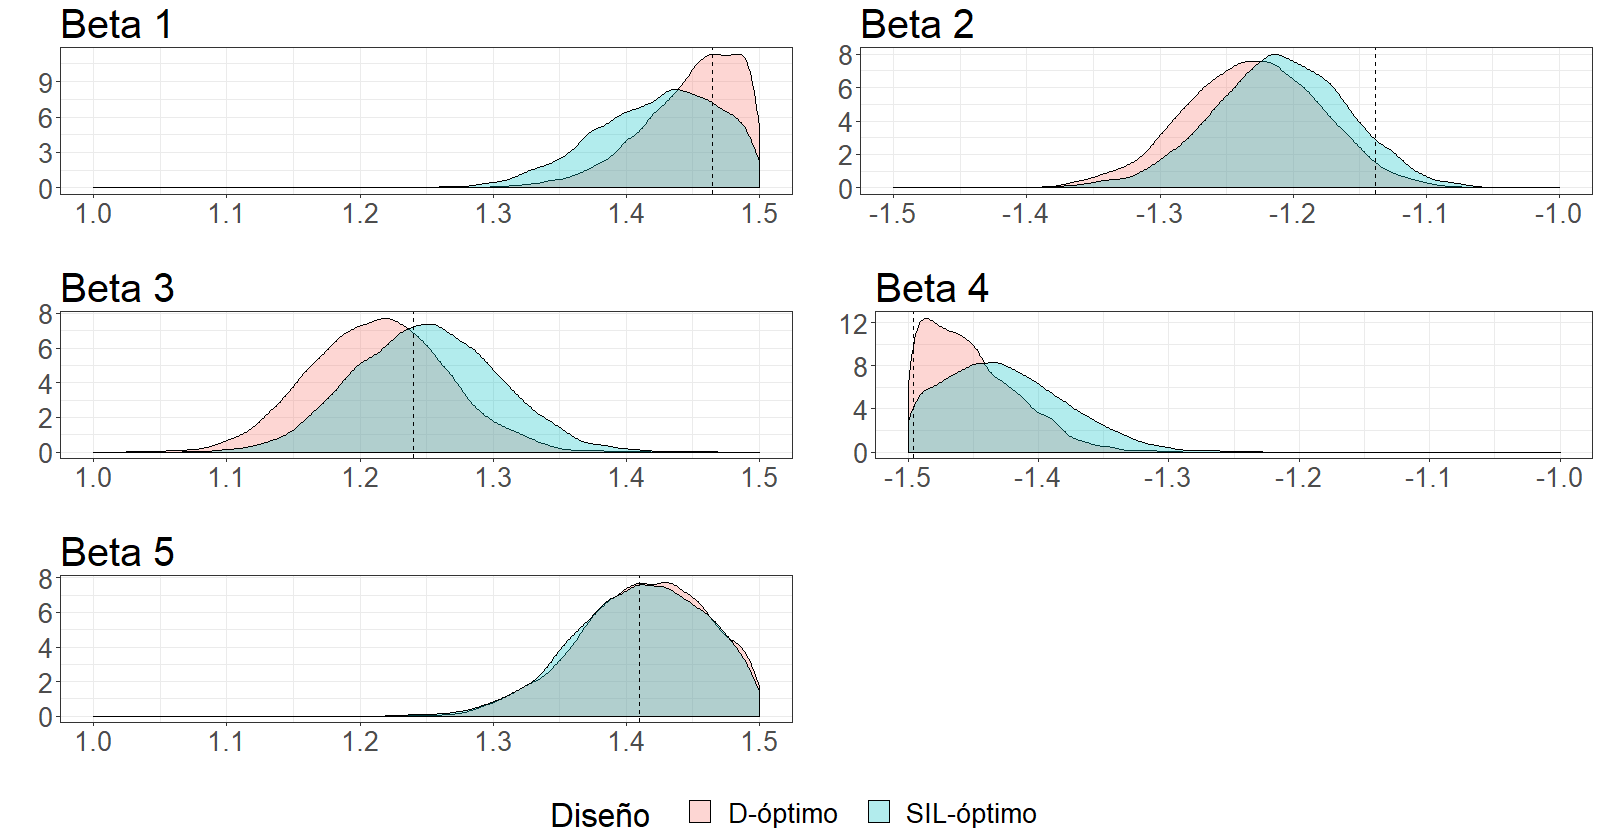
\includegraphics[width=\textwidth]{posterior_graphs_zoom.png}
    \caption{Densidades marginales posteriores de $\beta_1$, ..., $\beta_5$ derivadas de las series de datos $y_D$ e $y_{\text{SIL}}$. La línea punteada indica el valor simulado (\ref{eq:beta_sim}) del parámetro correspondiente.}
    \label{fig:posterior_beta}
\end{figure}



Por otro lado, en el ejemplo de la regresión logística las distribuciones iniciales de dos de los parámetros no contenían al cero en su soporte, ocasionando que se diera por hecho que ambos parámetros eran diferentes de cero. En este caso ocurre algo similar, solo que \textit{todos} los parámetros se suponen de dicha forma: para ambos valores de $\alpha$ (y para cualquier valor positivo de este parámetro, en realidad) las distribuciones iniciales no contienen al cero en su soporte. \\


De manera análoga al ejemplo anterior, se encontraron diseños óptimos pero habiendo modificado las distribuciones iniciales de forma que éstas sí contengan al cero en su soporte. En este caso, sin embargo, no solo se modificó el soporte de estas distribuciones, sino que además se escogió otra familia de distribuciones como sigue. Sea $\alpha > 0$ fijo. Las distribuciones iniciales propuestas por \cite{Woods_etal} (\ref{eq:mod2_params_initial}) se pueden clasificar en dos: aquellas que corresponden a $\beta_i$ con $i$ impar y aquellas que corresponden a $\beta_i$ con $i$ par. En el primer caso se considera una distribución uniforme en $(1, 1 + \alpha)$ y en el segundo una uniforme en $(-1 - \alpha, -1)$. Note que los autores suponen que todos los valores de $\beta$ son mayores que $-1 - \alpha$ y menores que $1 + \alpha$. \\


Se puede entonces pensar en una distribución inicial que, independientemente de si $i$ es par o impar, suponga que los parámetros se encuentran en el intervalo $(-1 - \alpha, 1 + \alpha)$. Además, para cambiar la familia de distribuciones y no solo el soporte, se puede utilizar alguna otra distribución que no sea uniforme. Para este propósito recordemos que la distribución Beta$(a, b)$ tiene soporte (0,1) y media igual a $a / (a + b)$. Luego, una variable aleatoria $X$ que siga una distribución Beta(2, 2) tendrá media igual a 1/2. Sea $Y = 2 (1 + \alpha) (X - \frac{1}{2})$ una transformación de la variable $X$. La función de densidad de $Y$ tiene la misma forma que la de $X$, pero con soporte igual al intervalo $(-1 - \alpha, 1 + \alpha)$. Se encontraron los diseños $D$-óptimos Bayesianos para $\alpha = 0.5$ y $\alpha = 0.75$ utilizando esta distribución como inicial para todos los parámetros. \\



Las Tablas \ref{table:alfa5_modified} y \ref{table:alfa75_modified} muestran la comparación del diseño SIL-óptimo con el $D$~-óptimo con las distribuciones iniciales modificadas y para $\alpha = 0.5$ y $\alpha = 0.75$, respectivamente. \\


\begin{table}[h]
\small
\centering
\begin{tabular}{l|lllll|lllll}
\multirow{2}{*}{Núm} & \multicolumn{5}{l|}{ \hspace{1.2cm} Diseño $D$~-óptimo} & \multicolumn{5}{l}{  \hspace{1cm}  Diseño SIL-óptimo}  \\
                     & $x_1$  & $x_2$ & $x_3$ & $x_4$ & $x_5$ & $x_1$ & $x_2$ & $x_3$ & $x_4$ & $x_5$  \\ \hline
1                    & 1  & 1    & 0.96     & -1    & 1     & -0.5  & -1    & 1     & -1    & 1      \\
2                    & 1      & 1  & 1     & 1    & -1     & 1     & 0.56  & 1     & -1    & 1      \\
3                    & -1      & -0.99    & -1  & -1    & -1     & 1     & -1    & -0.31 & -1    & 1      \\
4                    & -1      & 1    & -1     & 1  & 1     & 1     & -1    & 1     & 0.33  & 1      \\
5                    & 1      & -1    & -1     & 1    & 1 & 1     & -1    & 1     & -1    & -0.38 \\
6                    & -1      & -1    & 1     & 1    & 1     & 1     & -1    & 1     & -1    & 1     
\end{tabular}
\caption{Se muestran los diseños óptimos según los dos distintos criterios para $\alpha = 0.5$ y con las distribuciones iniciales modificadas.}
\label{table:alfa5_modified}
\end{table}



\begin{table}[h]
\small
\centering
\begin{tabular}{l|lllll|lllll}
\multirow{2}{*}{Núm} & \multicolumn{5}{l|}{ \hspace{1.2cm} Diseño $D$~-óptimo} & \multicolumn{5}{l}{  \hspace{1cm}  Diseño SIL-óptimo}  \\
                     & $x_1$  & $x_2$ & $x_3$ & $x_4$ & $x_5$ & $x_1$ & $x_2$ & $x_3$ & $x_4$ & $x_5$  \\ \hline
1                    & 1  & 1    & 1     & -1    & 1     & -0.22  & -1    & 1     & -1    & 1      \\
2                    & 1      & 1  & 1     & 1    & -1     & 1     & 0.22  & 1     & -1    & 1      \\
3                    & -1      & -1    & -1  & -1    & -1     & 1     & -1    & -0.32 & -1    & 1      \\
4                    & -1      & 1    & -1     & 1  & 1     & 1     & -1    & 1     & 0.11  & 1      \\
5                    & 1      & -1    & -1     & 1    & 1 & 1     & -1    & 1     & -1    & -0.31 \\
6                    & -1      & -1    & 1     & 1    & 1     & 1     & -1    & 1     & -1    & 1     
\end{tabular}
\caption{Se muestran los diseños óptimos según los dos distintos criterios para $\alpha = 0.75$ y con las distribuciones iniciales modificadas.}
\label{table:alfa75_modified}
\end{table}


Es evidente que los diseños óptimos bajo las nuevas distribuciones iniciales son diferentes a los diseños óptimos originalmente encontrados por \cite{Woods_etal} (y también a los diseños óptimos previamente encontrados). Primeramente, independientemente del valor de $\alpha$, ya no ocurre que todos los elementos de la matriz de diseño sean $\pm 1$ exceptuando a los elementos de la diagonal. Más aún, en el diseño con las iniciales originales todos los valores de cada covariable (cada columna) siempre valían lo mismo, excepto en un ensayo. En el caso de las iniciales modificadas lo que ocurre es que \textit{(i)} los elementos de la diagonal también valen $\pm 1$ y \textit{(ii)} las covariables ya no solo toman un valor (sin contar el valor de la diagonal que era distinto), sino que ahora valen 1 en algunos ensayos y -1 en otros. \\

Por otro lado al cambiar de $\alpha = 0.5$ a $\alpha = 0.75$ los diseños con las iniciales modificadas quedaron prácticamente iguales, salvo en dos entradas que son \textit{prácticamente} $\pm 1$. En resumen, la modificación de distribuciones iniciales introdujo cambios considerables en los diseño óptimos. \\


Por su parte, las Figuras \ref{fig:pois_reg5_modified} y \ref{fig:pois_reg75_modified} muestran las proyecciones en una y dos dimensiones de los diseños óptimos para $\alpha = 0.5$ y $\alpha = 0.75$, respectivamente (suavizando con un kernel Gaussiano para obtener la densidad de la proyección unidimensional).  \\

Algo interesante es que las correlaciones entre las covariables también cambiaron: si bien antes eran $\pm 0.2$ ahora no es así. En el caso de $\alpha = 0.5$ algunas correlaciones parecen estar alrededor de 1/3, otras alrededor de 0 y una última igual a 1/4. Esto se repite para el caso de $\alpha = 0.75$, donde además las correlaciones ya no están alrededor de estos valores sino que directamente eso valen. Puntualmente las correlaciones entre $x_1, x_2$ y $x_3$ son iguales a 1/3 y las respectivas a $x_4$ y $x_5$ con las demás covariables son 0, excepto precisamente por la correlación entre estas dos covariables, la cual toma el valor de 1/4. En resumen, pareciera que las covariables se separaron en dos grupos: $x_1, x_2$ y $x_3$ en un lado, correlacionadas entre sí por 1/3 pero no correlacionadas con las últimas dos covariables; y por otro lado $x_4$ y $x_5$, correlacionadas entre sí por 1/4 pero no correlacionadas con las primeras tres covariables.  \\



Finalmente las Figuras \ref{fig:pois_reg_conv_alfa5_modified} y \ref{fig:pois_reg_conv_alfa75_modified} muestran la evolución de la estimación de la pérdida esperada conforme el número de iteración avanza, para ambos valores de $\alpha$ respectivamente. En ambos casos la pérdida esperada parece haber convergido, por lo que se concluye lo mismo del método.




\begin{figure}[h]
	\centering
    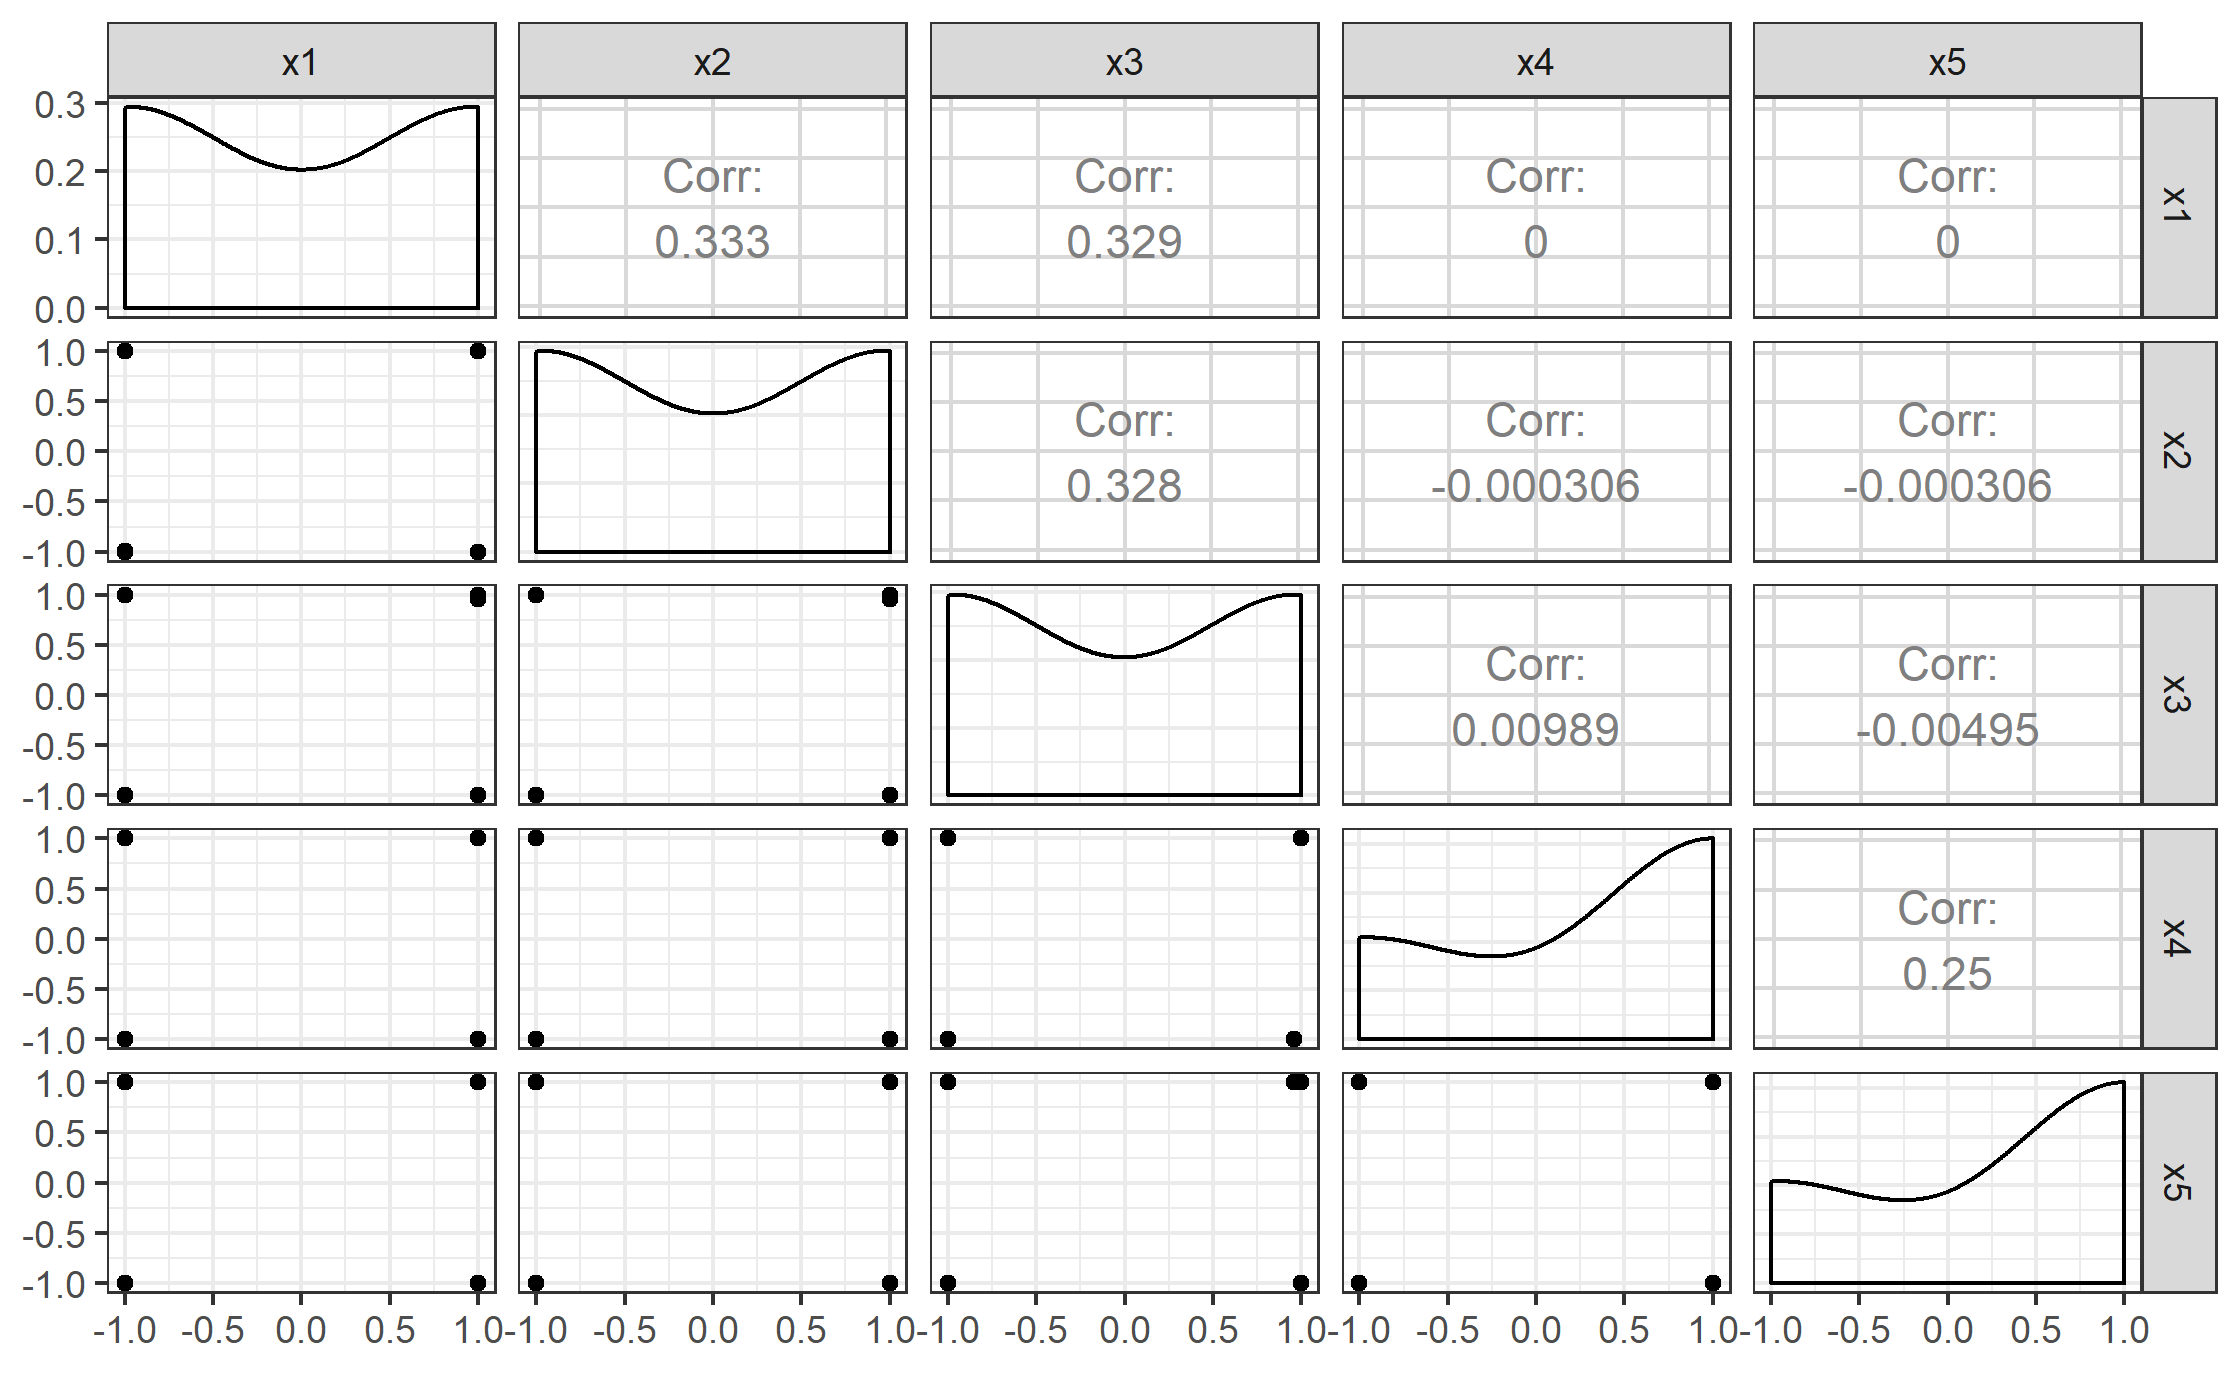
\includegraphics[width=\textwidth]{alpha_50_modified.png}
    \caption{Se muestran proyecciones en una y dos dimensiones de las tres variables del modelo de regresión Poisson (\ref{eq:mod2_poisson_regression1}) con distribuciones iniciales modificadas, así como su correlación, para $\alpha=0.5$.}
    \label{fig:pois_reg5_modified}
\end{figure}



\begin{figure}[h]
	\centering
    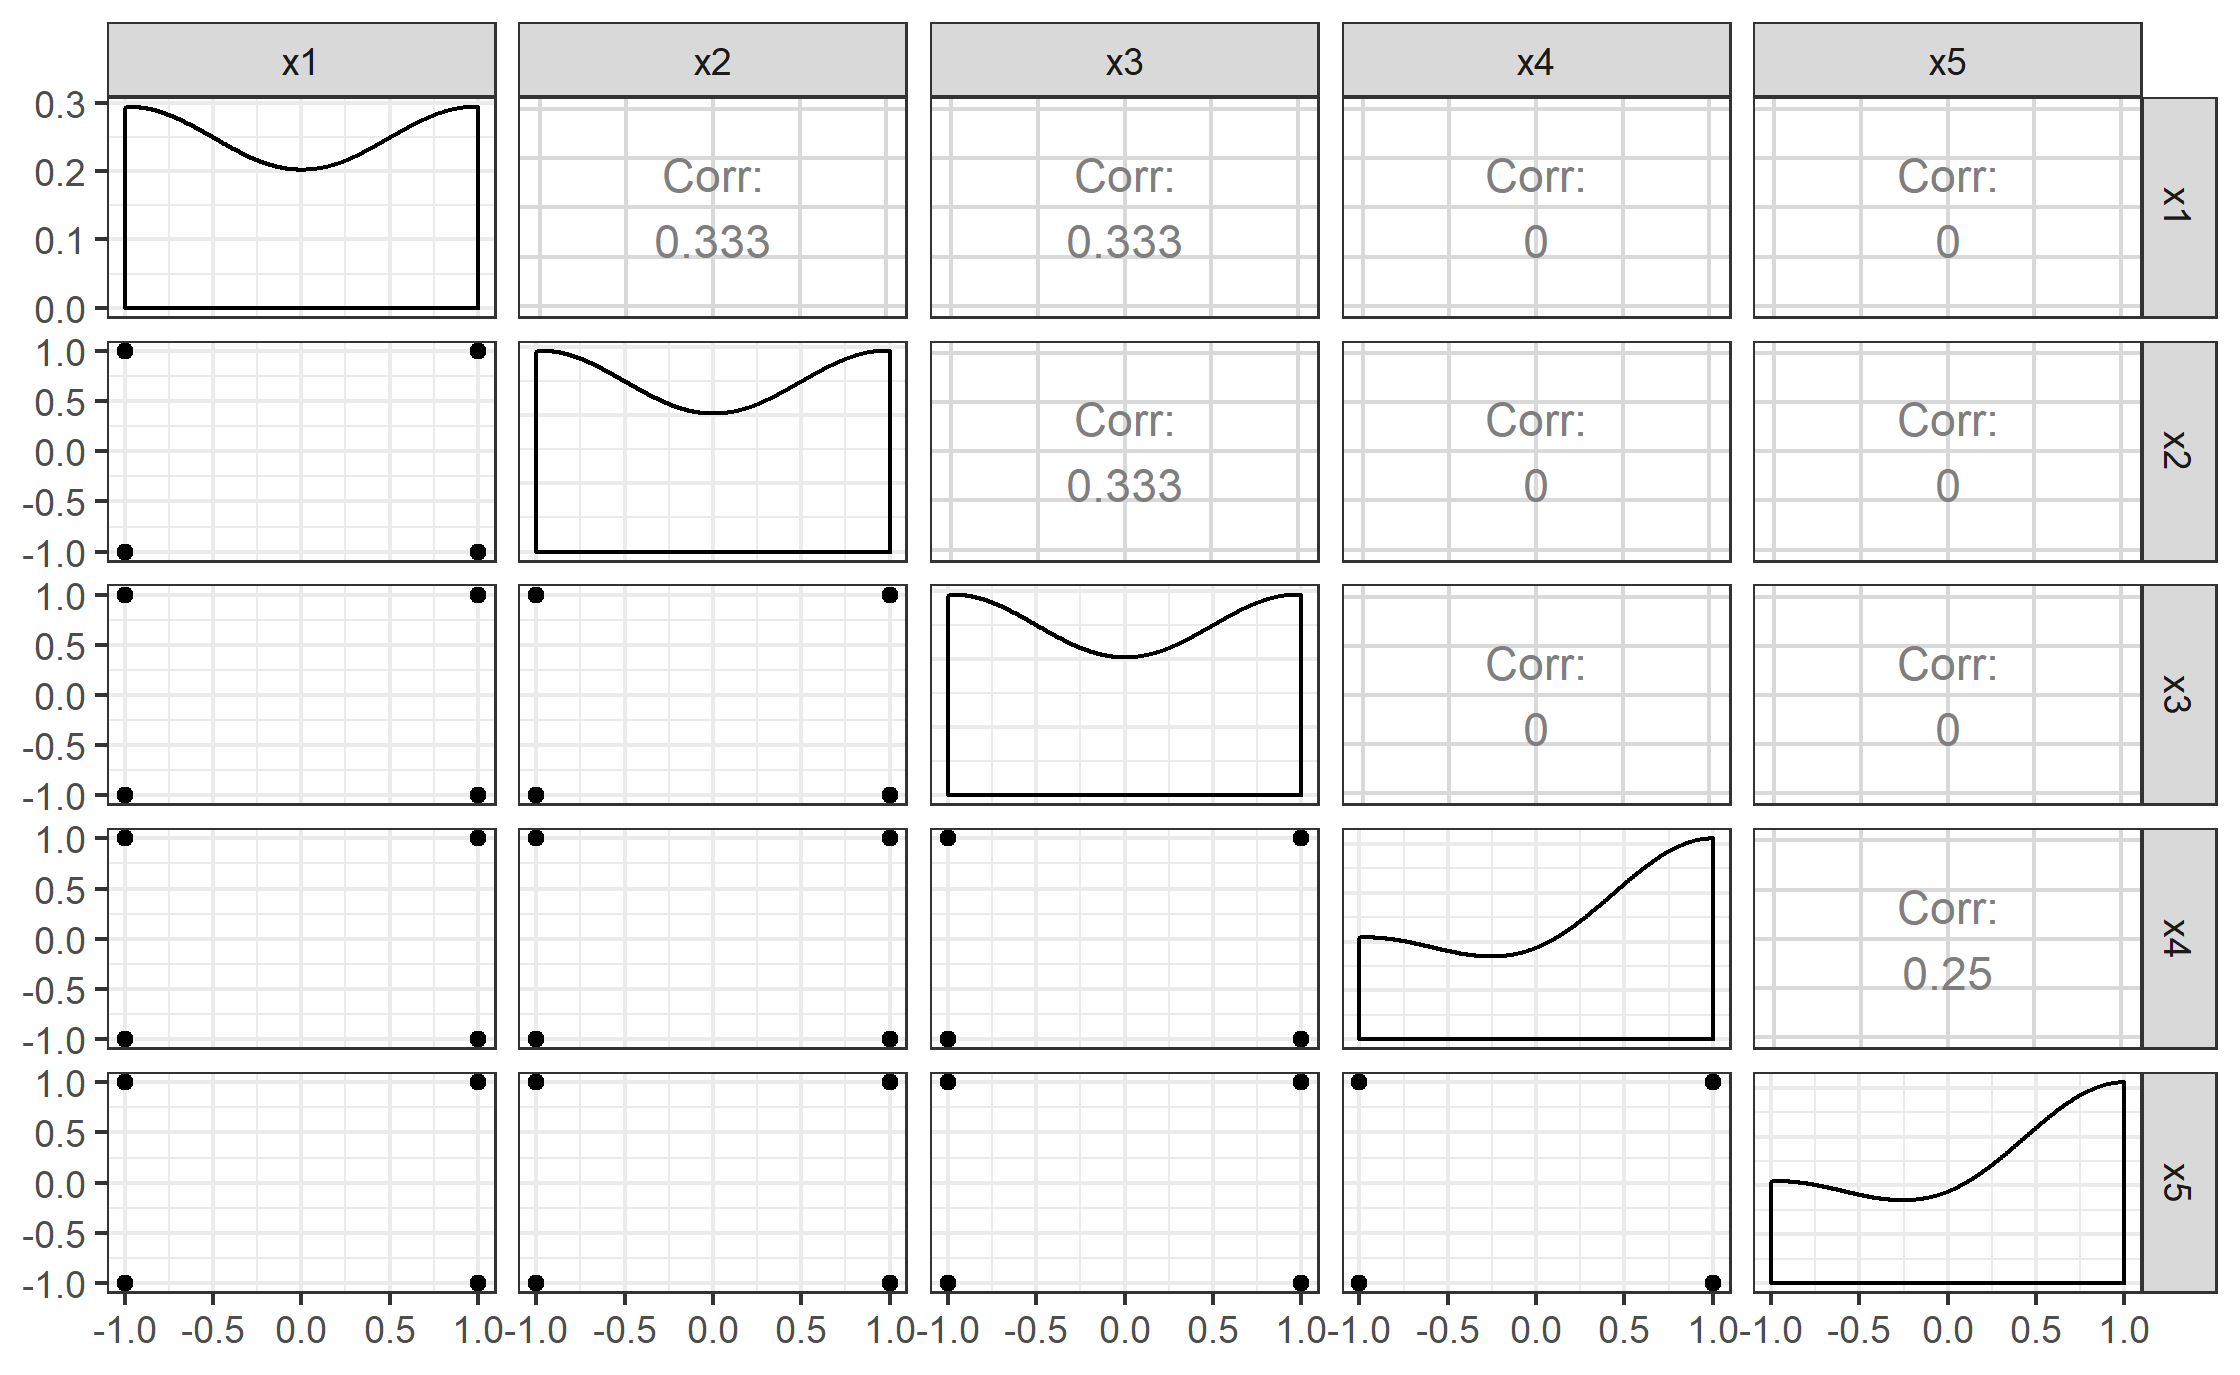
\includegraphics[width=\textwidth]{alpha_75_modified.png}
    \caption{Se muestran proyecciones en una y dos dimensiones de las tres variables del modelo de regresión Poisson (\ref{eq:mod2_poisson_regression1}) con distribuciones iniciales modificadas, así como su correlación, para $\alpha=0.75$.}
    \label{fig:pois_reg75_modified}
\end{figure}








\begin{figure}[h]
	\centering
    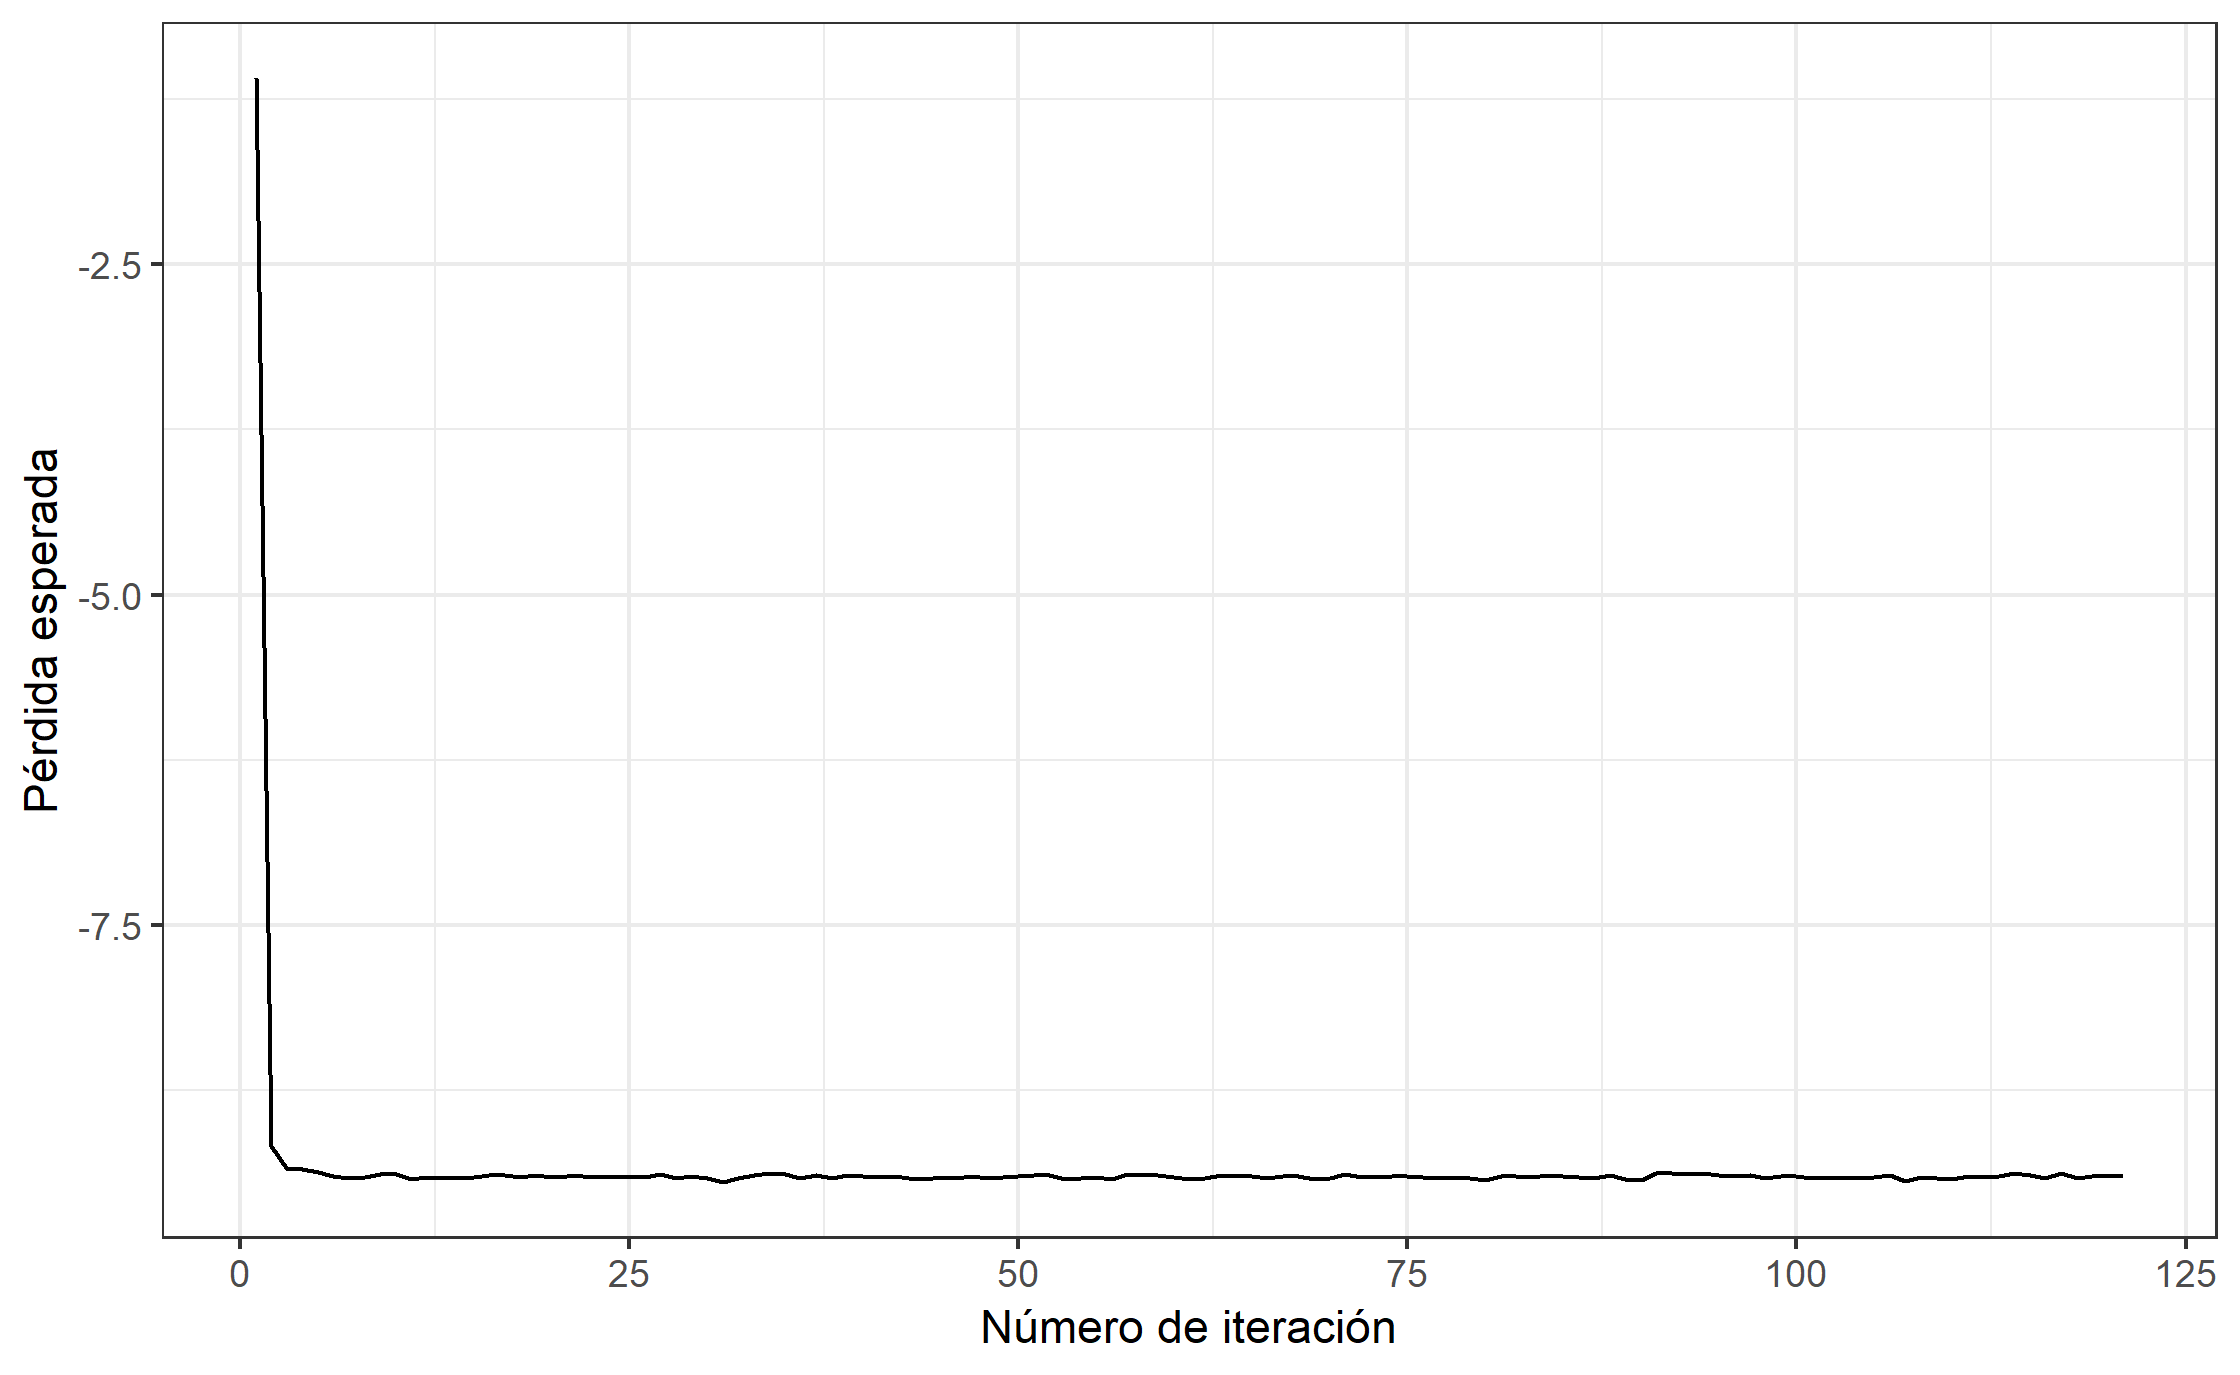
\includegraphics[width=\textwidth]{fig_conv_pois_reg_alfa5_modified.png}
    \caption{Para la regresión Poisson con distribuciones iniciales modificadas y $\alpha = 0.5$, se muestran aproximaciones a la utilidad esperada de los diseños en cada iteración del algoritmo para corroborar convergencia.}
    \label{fig:pois_reg_conv_alfa5_modified}
\end{figure}



\begin{figure}[h]
	\centering
    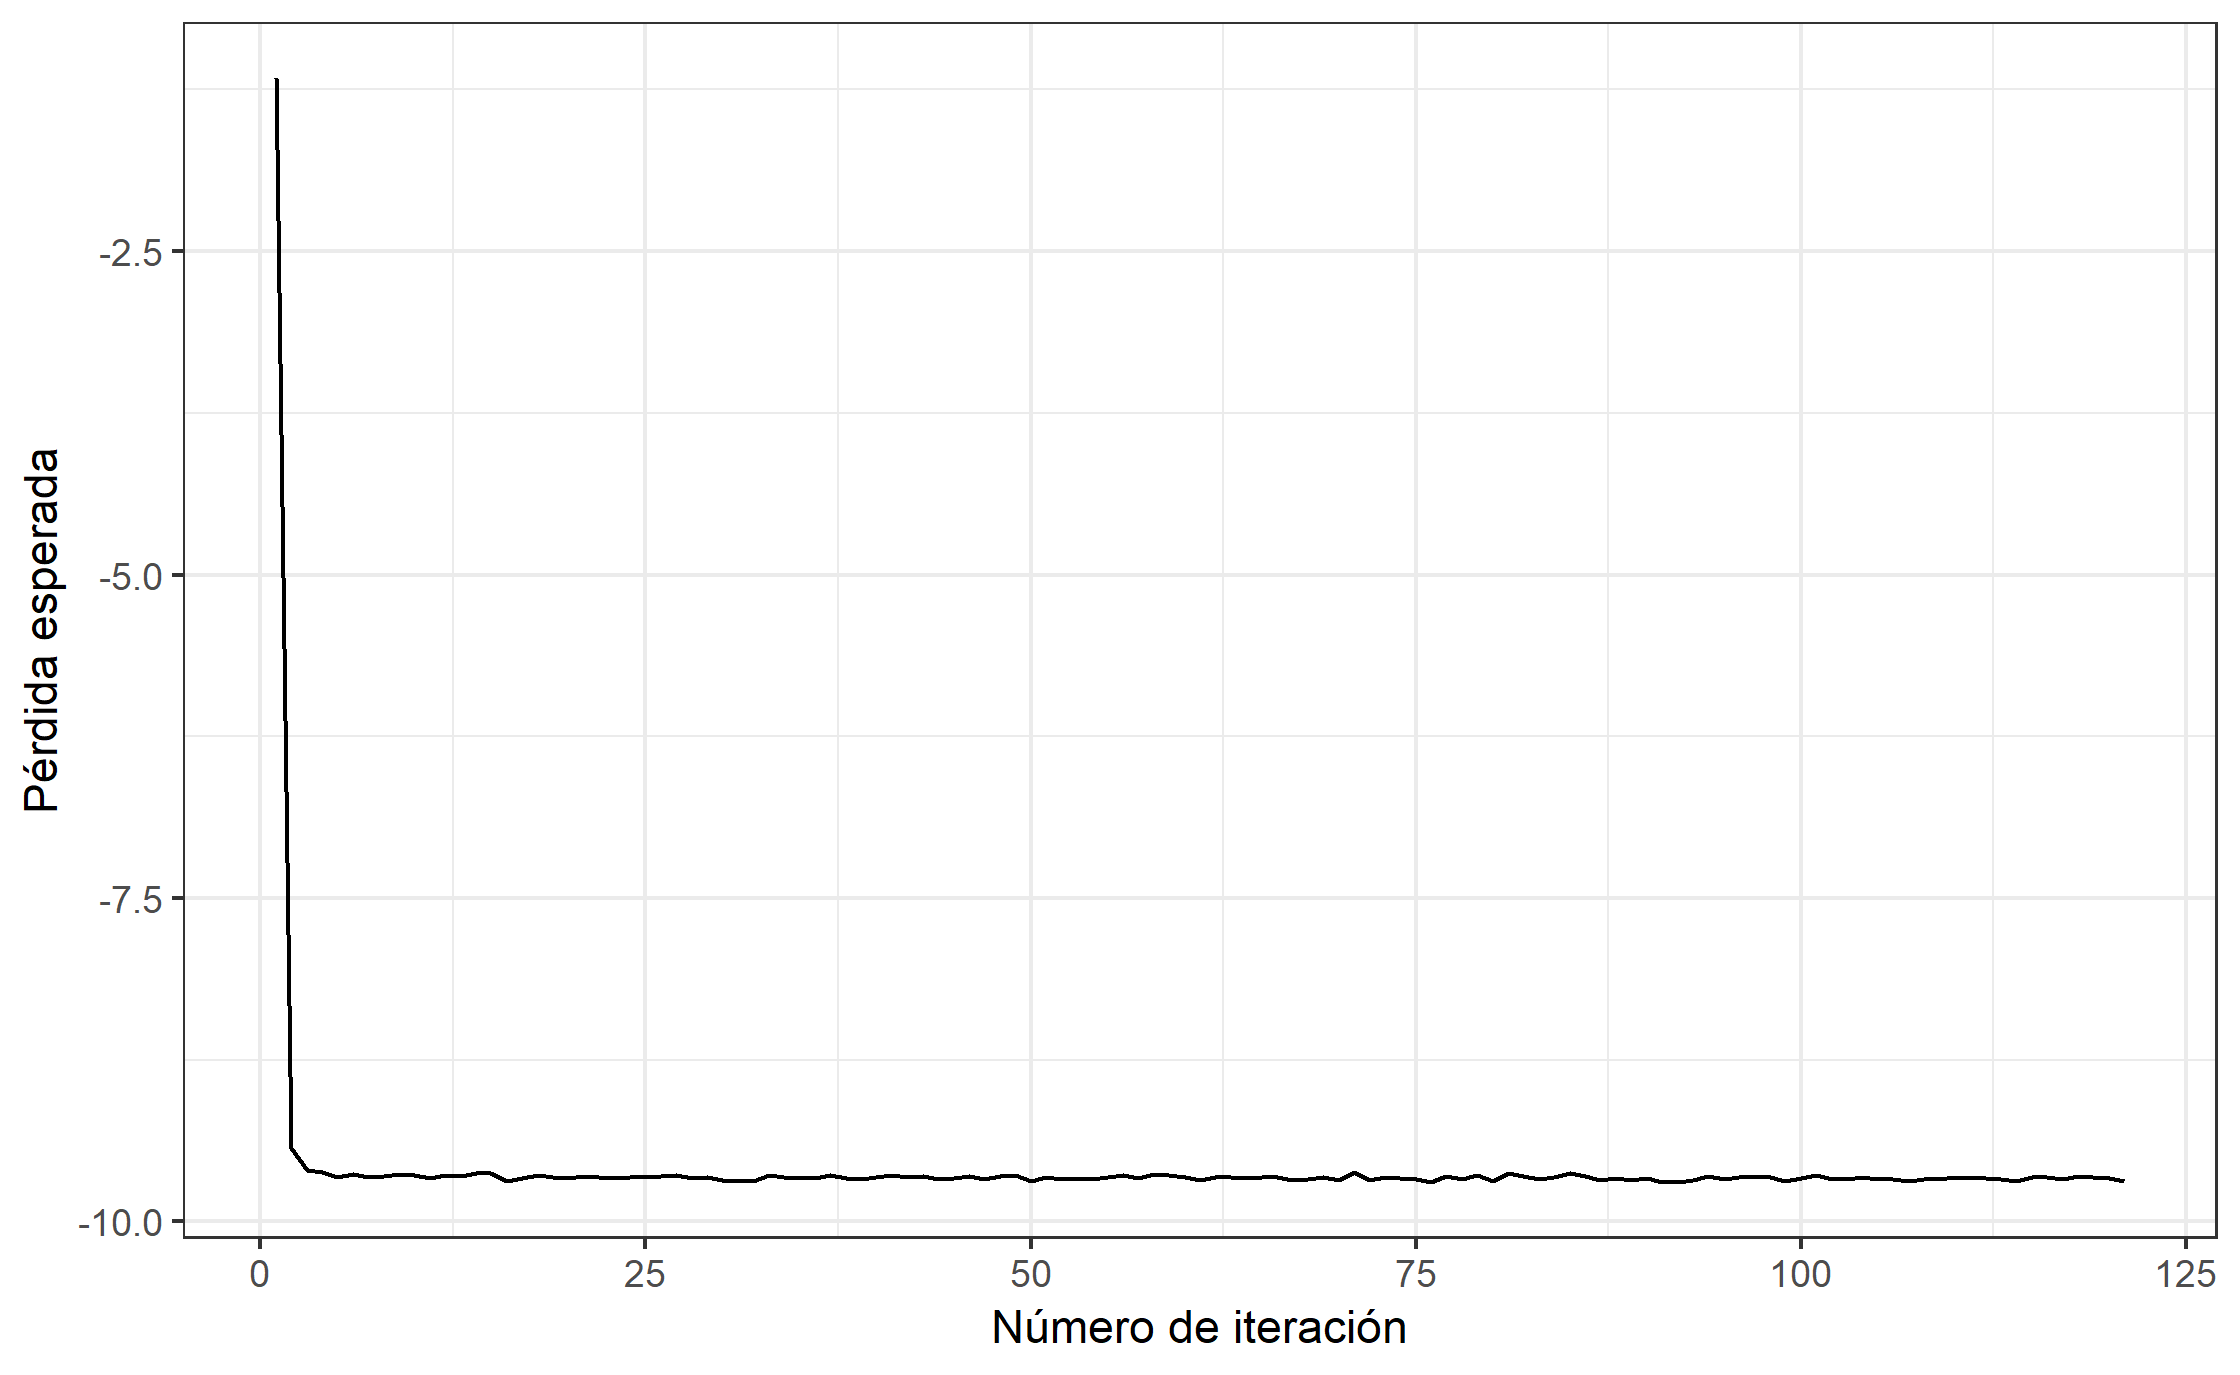
\includegraphics[width=\textwidth]{fig_conv_pois_reg_alfa75_modified.png}
    \caption{Para la regresión Poisson con distribuciones iniciales modificadas y $\alpha = 0.75$, se muestran aproximaciones a la utilidad esperada de los diseños en cada iteración del algoritmo para corroborar convergencia.}
    \label{fig:pois_reg_conv_alfa75_modified}
\end{figure}




\FloatBarrier






En el Apéndice \ref{chapter:appendixCode} se incluye el código utilizado para encontrar los diseños óptimos para cada uno de los ejemplos, así como para generar las gráficas aquí mostradas.










%\begin{figure}[h]
%\centering
%\begin{subfigure}{0.5\textwidth}
%  \centering
%  \includegraphics[scale=0.28]{pois_reg_alfa0_5}
%  \caption{$\alpha=0.5$.}
%  \label{fig:alfa.5}
%\end{subfigure}%
%\begin{subfigure}{0.5\textwidth}
%  \centering
%  \includegraphics[scale=0.28]{pois_reg_alfa0_75}
%  \caption{$\alpha=0.75$.}
%  \label{fig:alfa.75}
%\end{subfigure}
%\caption{Se muestran las proyecciones en una y dos dimensiones de las cinco %variables del modelo de regresión Poisson (\ref{eq:mod2_poisson_regression1}), así como su correlación, para los casos $\alpha = 0.5$ y $\alpha = 0.75$.}
%\label{fig:pois_reg}
%\end{figure}


%\section{Diseño para modelo de regresión Gamma}


%La distribución Gamma tiene la propiedad de ser sesgada a la derecha. Esto la hace sumamente útil para modelar fenómenos que sean no negativos y concentrados en una cierta región, pero que también produzcan datos atípicos. Uno puede pensar, por ejemplo, en el tiempo hasta que algún evento ocurra. Es en parte por ello que la distribución Gamma es popular en la práctica. En particular, es posible modelar respuestas que sigan dicha distribución mediante un modelo lineal generalizado. Como se menciona en el Apéndice \ref{chapter:appendixGLMs}, uno de los problemas es que la liga canónica es poco útil. La alternativa más popular, la liga logarítmica, ha dado buenos resultados y es bastante popular en la literatura. \\






